% ---------------------------------------------------------------------------------
% Main tex file
% $Id: Thesis.tex,v 1.2 2012/02/04 22:54:40 matsch Exp $

\documentclass[
a4,
oneside,
headsepline,     % Line under page header
normalheadings,
openany,
numbers=noenddot % Otherwise there will be a dot after the chapter numbering in case letters are used somewhere e.g. in the appendix
]{scrreprt} %report scrreprt
\setlength{\textwidth}{15cm}
\setlength{\textheight}{22.4cm}
%\oddsidemargin -0.1cm
%\evensidemargin 0.6cm

\usepackage[automark,headsepline]{scrpage2}
\pagestyle{scrheadings}
\clearscrheadfoot
\ihead{\headmark}
\ohead{\pagemark}
\cfoot{}
\setcounter{secnumdepth}{3}
\setcounter{tocdepth}{3}

% Alter some LaTeX defaults for better treatment of figures,
% from http://mintaka.sdsu.edu/GF/bibliog/latex/floats.html
% See p.105 of "TeX Unbound" for suggested values.
% See pp. 199-200 of Lamport's "LaTeX" book for details.
% General parameters, for ALL pages:
\renewcommand{\topfraction}{0.9}	% max fraction of floats at top
\renewcommand{\bottomfraction}{0.8}	% max fraction of floats at bottom
% Parameters for TEXT pages (not float pages):
%\setcounter{topnumber}{2}
%\setcounter{bottomnumber}{2}
%\setcounter{totalnumber}{4}     % 2 may work better
%\setcounter{dbltopnumber}{2}    % for 2-column pages
\renewcommand{\dbltopfraction}{0.9}	% fit big float above 2-col. text
\renewcommand{\textfraction}{0.07}	% allow minimal text w. figs
% Parameters for FLOAT pages (not text pages):
\renewcommand{\floatpagefraction}{0.7}	% require fuller float pages
% N.B.: floatpagefraction MUST be less than topfraction !!
\renewcommand{\dblfloatpagefraction}{0.7}	% require fuller float pages
% remember to use [htp] or [htpb] for placement



\usepackage{amsfonts}
\usepackage{amsmath}  % Correct size switching in mathmode when using \text{} instead of \textrm{}
\usepackage{amssymb} 
\usepackage{amstext} 
\usepackage{multirow}
\usepackage{longtable}
\usepackage{cite}
\usepackage{graphicx}
\usepackage{booktabs}

% ---------------------------------------------------------------------------------
% Collection of user-defined commands
% $Id: definitions.tex,v 1.3 2012/02/05 21:33:26 matsch Exp $

\usepackage{amsmath}
\usepackage{xspace}

\newcommand{\tobechecked}{\textcolor{red}{\textbf{(to be checked)}}}
\newcommand{\alreadydefined}[1]{\textcolor{red}{\textbf{(#1 already defined?)}}}
\newcommand{\todo}[1]{\textcolor{blue}{{\textbf{TODO: }\textit{#1}}}}
\newcommand{\fixme}[1]{\textcolor{red}{{\textbf{FIXME: }\textit{#1}}}}
\newcommand{\addref}{\textcolor{blue}{ADD REFERENCE}}
\newcommand{\addfig}[1]{\textcolor{red}{\textbf{ADD FIGURE: }\textit{#1}}}

% Sectioning
\newcommand{\qsec}[1]{Section~\ref{#1}}
\newcommand{\qsecs}[2]{Sections~\ref{#1} and~\ref{#2}}
\newcommand{\cfqsec}[1]{cf.\ Section~\ref{#1}}
\newcommand{\qfig}[1]{Fig.~\ref{#1}}
\newcommand{\qfigs}[2]{Figs.~\ref{#1} and~\ref{#2}}
\newcommand{\cfqfig}[1]{cf.\ Fig.~\ref{#1}}
\newcommand{\qsubfig}[2]{Fig.~\ref{#1}~(\textit{#2})}
\newcommand{\qtab}[1]{Table~\ref{#1}}
\newcommand{\qtabs}[2]{Tables~\ref{#1} and~\ref{#2}}
\newcommand{\cfqtab}[1]{cf.\ Table~\ref{#1}}
\newcommand{\qeq}[1]{\eqref{#1}}

% Units
\newcommand{\tev}{\ensuremath{\;\text{Te}\kern-0.06667em\text{V}}\xspace}
\newcommand{\gev}{\ensuremath{\;\text{Ge}\kern-0.06667em\text{V}}\xspace}
\newcommand{\mev}{\ensuremath{\;\text{Me}\kern-0.06667em\text{V}}\xspace}
\newcommand{\kev}{\ensuremath{\;\text{ke}\kern-0.06667em\text{V}}\xspace}
\newcommand{\ev}{\ensuremath{\;\text{e}\kern-0.06667em\text{V}}\xspace}
\newcommand{\tevnospace}{\ensuremath{\text{Te}\kern-0.06667em\text{V}}\xspace}
\newcommand{\gevnospace}{\ensuremath{\text{Ge}\kern-0.06667em\text{V}}\xspace}
\newcommand{\mevnospace}{\ensuremath{\text{Me}\kern-0.06667em\text{V}}\xspace}
\newcommand{\kevnospace}{\ensuremath{\text{ke}\kern-0.06667em\text{V}}\xspace}
\newcommand{\evnospace}{\ensuremath{\text{e}\kern-0.06667em\text{V}}\xspace}
\newcommand{\km}{\ensuremath{\;\text{km}}\xspace}
\newcommand{\m}{\ensuremath{\;\text{m}}\xspace}
\newcommand{\cm}{\ensuremath{\;\text{cm}}\xspace}
\newcommand{\mm}{\ensuremath{\;\text{mm}}\xspace}
\newcommand{\second}{\ensuremath{\;\text{s}}\xspace}
\newcommand{\kg}{\ensuremath{\;\text{kg}}\xspace}
\newcommand{\tons}{\ensuremath{\;\text{t}}\xspace}
\newcommand{\tesla}{\ensuremath{\;\text{T}}\xspace}
\newcommand{\kelvin}{\ensuremath{\;\text{K}}\xspace}
\newcommand{\nbinv}{\ensuremath{\;\text{nb}^{-1}}\xspace}
\newcommand{\pbinv}{\ensuremath{\;\text{pb}^{-1}}\xspace}
\newcommand{\fbinv}{\ensuremath{\;\text{fb}^{-1}}\xspace}

% Quantities
\newcommand{\et}{\ensuremath{E_{\text{T}}}\xspace}
\newcommand{\met}{\ensuremath{\slash\mkern-12mu{E}_{\text{T}}}\xspace}
\newcommand{\metvec}{\ensuremath{\slash\mkern-12mu{\vec{E}}_{\text{T}}}\xspace}
\newcommand{\HT}{\ensuremath{H_{\text{T}}}\xspace}
\newcommand{\HTvec}{\ensuremath{\vec{H}_{\text{T}}}\xspace}
\newcommand{\MHT}{\ensuremath{\slash\mkern-12mu{H}_{\text{T}}}\xspace}
\newcommand{\MHTvec}{\ensuremath{\slash\mkern-12mu{\vec{H}}_{\text{T}}}\xspace}
\newcommand{\pt}{\ensuremath{p_{\text{T}}}\xspace}
\newcommand{\ptvec}{\ensuremath{\vec{p}_{\text{T}}}\xspace}
\newcommand{\pti}[1]{\ensuremath{p_{\text{T},#1}}\xspace}
\newcommand{\ptivec}[1]{\ensuremath{\vec{p}_{\text{T},#1}}\xspace}
\newcommand{\ptsub}[1]{\ensuremath{p_{\text{T},#1}}\xspace}
\newcommand{\ptvecsub}[1]{\ensuremath{\vec{p}_{\text{T},#1}}\xspace}
\newcommand{\ptdijet}{\ensuremath{p^{\text{dijet}}_{\text{T}}}\xspace}
\newcommand{\ptave}{\ensuremath{p^{\text{ave}}_{\text{T}}}\xspace}
\newcommand{\ptavei}[1]{\ensuremath{p^{\text{ave}}_{\text{T,#1}}}\xspace}
\newcommand{\ptavemin}{\ensuremath{p^{\text{ave,min}}_{\text{T}}}\xspace}
\newcommand{\ptavemax}{\ensuremath{p^{\text{ave,max}}_{\text{T}}}\xspace}
\newcommand{\ptgen}{\ensuremath{p^{\text{gen}}_{\text{T}}}\xspace}
\newcommand{\ptgenave}{\ensuremath{p^{\text{gen,ave}}_{\text{T}}}\xspace}
\newcommand{\ptgenrel}{\ensuremath{p^{\text{gen,rel}}_{\text{T,3}}}\xspace}
\newcommand{\ptgeni}[1]{\ensuremath{p^{\text{gen}}_{\text{T},#1}}\xspace}
\newcommand{\ptgenivec}[1]{\ensuremath{\vec{p}^{\text{gen}}_{\text{T},#1}}\xspace}
\newcommand{\pthat}{\ensuremath{\hat{p}_{\text{T}}}\xspace}
\newcommand{\pthatmin}{\ensuremath{\hat{p}^{\text{min}}_{\text{T}}}\xspace}
\newcommand{\pthatmax}{\ensuremath{\hat{p}^{\text{max}}_{\text{T}}}\xspace}
\newcommand{\pttrue}{\ensuremath{p^{\text{true}_{}}_{\text{T}}}\xspace}
\newcommand{\pttruei}[1]{\ensuremath{p^{\text{true}_{}}_{\text{T,}#1}}\xspace}
\newcommand{\ptreco}{\ensuremath{p^{\text{reco}_{}}_{\text{T}}}\xspace}
\newcommand{\ptrel}{\ensuremath{p^{\text{rel}_{}}_{\text{T},3}}\xspace}
\newcommand{\ptmin}{\ensuremath{p^{\text{min}_{}}_{\text{T}}}\xspace}
\newcommand{\ptmax}{\ensuremath{p^{\text{max}_{}}_{\text{T}}}\xspace}
\newcommand{\ptparticle}{\ensuremath{p^{\text{particle}_{}}_{\text{T}}}\xspace}
\newcommand{\ptparton}{\ensuremath{p^{\text{parton}_{}}_{\text{T}}}\xspace}
\newcommand{\ptref}{\ensuremath{p^{\text{ref}_{}}_{\text{T}}}\xspace}
\newcommand{\ppgen}{\ensuremath{p^{\text{gen}}_{||}}\xspace}
\newcommand{\ppgeni}[1]{\ensuremath{p^{\text{gen}}_{||,#1}}\xspace}
\newcommand{\ppi}[1]{\ensuremath{p_{||,#1}}\xspace}
\newcommand{\ptimbal}{\ensuremath{p_{\text{T,imbal}}}\xspace}
\newcommand{\ptimbalrel}{\ensuremath{p^{\text{rel}}_{\text{T,imbal}}}\xspace}
\newcommand{\etamin}{\ensuremath{\eta^{\text{min}}}\xspace}
\newcommand{\etamax}{\ensuremath{\eta^{\text{max}}}\xspace}
\newcommand{\etagen}{\ensuremath{\eta^{\text{gen}}}\xspace}
\newcommand{\alphat}{\ensuremath{\alpha_{\text{T}}}\xspace}
\newcommand{\planckscl}{\ensuremath{\Lambda_{\text{P}}}\xspace}
\newcommand{\xtrue}{\ensuremath{x^{\text{true}}}\xspace}
\newcommand{\meanxtrue}{\ensuremath{\bar{x}^{\text{true}}}\xspace}
\newcommand{\xmeasi}[1]{\ensuremath{x_{#1}}\xspace}
\newcommand{\xave}{\ensuremath{x^{\text{ave}}}\xspace}

% Symbols
\newcommand{\dif}[1]{\ensuremath{\text{d}#1}\xspace}
\newcommand{\e}{\,\text{e}}
\newcommand{\nup}[1]{$^{\text{\scriptsize #1}}$}
\newcommand{\dgr}{\ensuremath{\,^{\circ}}}
\newcommand{\mean}[1]{\ensuremath{\langle#1\rangle}}
\newcommand{\gqq}[1]{\ensuremath{\glqq#1\grqq}}
\newcommand{\rarr}{\ensuremath{\rightarrow}\xspace}
\newcommand{\ket}[1]{\ensuremath{\left|#1\right>}\xspace}
\newcommand{\bra}[1]{\ensuremath{\left<#1\right|}\xspace}
\newcommand{\bracket}[2]{\ensuremath{\left<#2\right|#1\left|#2\right>}\xspace}

% Particles
\newcommand{\lel}{\ensuremath{e}\xspace}
\newcommand{\lelr}{\ensuremath{e_{R}}\xspace}
\newcommand{\lmu}{\ensuremath{\mu}\xspace}
\newcommand{\ltau}{\ensuremath{\tau}\xspace}
\newcommand{\nue}{\ensuremath{\nu_{e}}\xspace}
\newcommand{\nuer}{\ensuremath{\nu_{e,R}}\xspace}
\newcommand{\numu}{\ensuremath{\nu_{\mu}}\xspace}
\newcommand{\nutau}{\ensuremath{\nu_{\tau}}\xspace}
\newcommand{\qu}{\ensuremath{u}\xspace}
\newcommand{\qd}{\ensuremath{d}\xspace}
\newcommand{\qc}{\ensuremath{c}\xspace}
\newcommand{\qs}{\ensuremath{s}\xspace}
\newcommand{\qt}{\ensuremath{t}\xspace}
\newcommand{\qb}{\ensuremath{b}\xspace}
\newcommand{\photon}{\ensuremath{\gamma}\xspace}
\newcommand{\Z}{\ensuremath{Z^{0}}\xspace}
\newcommand{\W}{\ensuremath{W^{\pm}}\xspace}
\newcommand{\Wp}{\ensuremath{W^{+}}\xspace}
\newcommand{\Wm}{\ensuremath{W^{-}}\xspace}

% Processes
\newcommand{\ZInv}{\ensuremath{Z\rightarrow\nu\bar{\nu}}\xspace}
\newcommand{\ZInvJets}{\ZInv+jets\xspace}
\newcommand{\ttbar}{\ensuremath{t\bar{t}}\xspace}
\newcommand{\WJets}{\ensuremath{W}+jets\xspace}

% Programmes
\newcommand{\isajet}{\textsc{IsaJet}\xspace}
\newcommand{\madgraph}{\textsc{Madgraph}\xspace}
\newcommand{\prospino}{\textsc{Prospino}\xspace}
\newcommand{\pythia}{\textsc{Pythia}\xspace}
\newcommand{\herwig}{\textsc{Herwig++}\xspace}
\newcommand{\geant}{\textsc{GEANT4}\xspace}

% Experiments and facilities
\newcommand{\lhc}{LHC\xspace}
\newcommand{\cms}{CMS\xspace}
\newcommand{\dzero}{D\O\xspace}

% Other words and characters
\newcommand{\sm}{SM\xspace}
\newcommand{\susy}{SUSY\xspace}
\newcommand{\mssm}{MSSM\xspace}
\newcommand{\cmssm}{CMSSM\xspace}
\newcommand{\lsp}{LSP\xspace}
\newcommand{\dm}{DM\xspace}
\newcommand{\de}{DE\xspace}
\newcommand{\CLs}{\ensuremath{\text{CL}_{s}}\xspace}
\newcommand{\CL}{\ensuremath{\text{CL}}\xspace}
\newcommand{\cp}{CP\xspace}
\newcommand{\ratwo}{jets+met\xspace}
\newcommand{\hadtau}{hadronic-$\tau$\xspace}
\newcommand{\lostlep}{lost-lepton\xspace}
\newcommand{\PF}{PF\xspace}
\newcommand{\calo}{Calo jets\xspace}
\newcommand{\jpt}{JPT jets\xspace}
\newcommand{\pf}{PF jets\xspace}
\newcommand{\antikt}{anti-$k_{T}$\xspace}
\newcommand{\resp}{\ensuremath{\mathcal{R}}\xspace}
\newcommand{\asym}{\ensuremath{\mathcal{A}}\xspace}
\newcommand{\lvmini}{\textsc{LVMINI}\xspace}
\newcommand{\corescale}{\ensuremath{\lambda_{\text{res}}}\xspace}

% Symbols for tail studies
\newcommand{\fasym}{\ensuremath{f_{\text{asym}}}\xspace}
\newcommand{\fasymdata}{\ensuremath{f^{\text{data}}_{\text{asym}}}\xspace}
\newcommand{\fasymmc}{\ensuremath{f^{\text{mc}}_{\text{asym}}}\xspace}
\newcommand{\fasymtoy}{\ensuremath{f^{\text{toy}}_{\text{asym}}}\xspace}
\newcommand{\fresp}{\ensuremath{f_{\text{resp}}}\xspace}
\newcommand{\frespdata}{\ensuremath{f^{\text{data}}_{\text{resp}}}\xspace}
\newcommand{\frespmc}{\ensuremath{f^{\text{mc}}_{\text{resp}}}\xspace}
\newcommand{\fresptoy}{\ensuremath{f^{\text{toy}}_{\text{resp}}}\xspace}
\newcommand{\window}[1]{\ensuremath{>#1\,\sigma_{A}}}
\newcommand{\windowexcl}[2]{\ensuremath{#1-#2\,\sigma_{A}}}
\newcommand{\windowinf}[1]{\ensuremath{#1\,\sigma_{A} - \infty}}

% Abbrevations
\newcommand{\etc}{e.\,t.\,c.\ }
\newcommand{\wrt}{w.\,r.\,t.\ }
\newcommand{\cf}{cf.\ }
\newcommand{\ie}{i.\,e.\ }
\newcommand{\siehe}{s.\ }
\newcommand{\zb}{z.\,B.\ }
\newcommand{\ca}{ca.\ }
\newcommand{\eg}{e.\,g.\ }
\newcommand{\vs}{vs.\ }

% Constants
\newcommand{\lumiratwo}{\ensuremath{1.1\fbinv}\xspace}
\newcommand{\lumires}{\ensuremath{0.84\fbinv}\xspace}


\title{Measurement of the Jet Transverse Momentum Resolution and Response Tails and Application in a QCD Background Estimation Method in a Search for New Physics at CMS}
\author{Matthias Schr\"oder}

% pdflatex packages
\usepackage[pdftex]{hyperref}
\hypersetup{bookmarks=true}
\hypersetup{unicode=true}
\hypersetup{colorlinks=true,%
  citecolor=black,%
  filecolor=black,%
  linkcolor=black,%
  urlcolor=black}
\hypersetup{pdftitle={Search for Supersymmetry in All-Hadronic Final States at CMS}}
\hypersetup{pdfauthor={Matthias Schr\"oder}}

\begin{document}
\maketitle
\tableofcontents

\chapter{Introduction}


\chapter{The standard model and super symmetry}
%% ---------------------------------------------------------------------------------
% Chapter: Theory
% $Id: Theory.tex,v 1.2 2012/02/04 22:54:40 matsch Exp $

In this chapter, an introduction is provided to the theoretical background in particle physics relevant for this thesis.
First in \qsec{sec:Theory:SM}, the \emph{Standard Model} (`\sm') of particle physics is presented, which comprises the most advanced description of the fundamental constituents and interactions in nature based on fundamental symmetry principles and only a limited number of parameters.
The \sm has been remarkably successful and experimentally verified to an extremely high precision\todo{put some meaningful number} over a wide range of energies from a few \evnospace to the \tevnospace scale, making the \sm one of the most successful scientific theories ever developed.
However, there are a number of observations in tension to its predictions, as discussed in \qsec{sec:Theory:BeyondSM}.
For example, neither can the masses of particles or the resulting gravitational interactions be described in the \sm, nor does it include candidates for \emph{Dark Matter} or \emph{Dark Energy}, which are assumed to constitute most of the energy density in the universe.
Furthermore, radiative corrections to certain processes become divergent at high energies resulting in a violation of unitarity.
This and other theoretical considerations clearly point to the limited validity of the \sm.
Therefore, possible extensions to the \sm, which can provide solutions to several of the above problems, are outlined.
In particular, the concept of \emph{Supersymmetry} is introduced and discussed in greater detail in \qsec{sec:Theory:SUSY}.



\section{The Standard Model of Particle Physics}\label{sec:Theory:SM}
\subsection{Introduction}
Already about 2400 years ago\footnote{It's a warm summer evening, circa $400\;\text{BC}$\ldots}, Democritus and Leucippus hypothesised~\cite{bib:Stoerig:Philosophie} that everything in the universe is composed of indivisible units (`\'{a}tomos'), a concept still present in the modern picture of nature.
The \sm of particle physics describes \emph{quarks} (`q') and \emph{leptons} as fundamental constituents of matter.
They can be interpreted as structureless fermions, \ie particles with spin~$1/2$, which have further properties such as charge or mass generally denoted as \emph{quantum numbers}.
Their dynamics are completely determined by a small set of fundamental interactions, from which -- at least in principle -- all other laws of physics\footnote{This does not hold true for gravity-related processes, since gravity cannot be incorporated consistently into the \sm.} can be derived.
In the \sm, three fundamental interactions are described: the \emph{electromagnetic}, the \emph{weak}, and the \emph{strong interaction}.
These interactions, \ie the transfer of energy and momentum as well as the alteration of quantum numbers, are mediated by the exchange of other elementary particles, bosons, which carry spin $1$.
The strength of the interactions depends on the fermion charges, which act as \emph{coupling constants} and determine the probability of a fermion emitting or absorbing a boson.

Mathematically, the \sm is based on quantum field theories, which incorporate special relativity and quantum mechanics.
The matter fermions are represented by states of quantised spinor fields, the exchange bosons by states of quantised vector fields in Fock space.
All information about a system is encoded in the \emph{Lagrangian} $\mathcal{L}$, a scalar function of the fields.
Much in analogy to classical mechanics, the equations of motion of the fields can be obtained from $\mathcal{L}$ when assuming the principle of stationary action \mbox{$\delta S = 0$}, where the action $S$ is defined as
\begin{equation*}
  S = \int\dif{t}\;\mathcal{L} \;,
\end{equation*}
with $t$ denoting time.
The resulting equations of motion are the Dirac equation for fermions and the Klein-Gordon equation for bosons.
Astonishingly, the interaction terms of the \sm are introduced naturally when assuming local invariance of $\mathcal{L}$ under certain unitary transformation (\emph{gauge transformations}).

The equations of motion can in general not be solved analytically for non-trivial systems of interacting particles.
It is possible, however, to expand the solution in orders of the coupling constants.
Each term in this \emph{perturbation series} can be associated with a certain physical process contributing to the total interaction.
Although usually terms can only be computed to the first few orders, this provides an adequate approximation of the interaction probability since the coupling constants are small (except for low energy processes of the strong interaction).
\todo{Need to introduce / mention renormalisation, running couplings because mentioned later.}

The gauge invariance of the Lagrangian will be discussed in more detail later in \qsec{sec:Theory:SM:GaugeInteractions}; first, a more phenomenological overview of the \sm will be given.
A detailed introduction to the \sm and the underlying gauge-principles is given for instance in~\cite{bib:Schmuser:FeynmanGraphs,bib:AitchisonHey:GaugeTheories1,bib:AitchisonHey:GaugeTheories2}, an introduction to quantum field theory in general in~\cite{bib:MandlShaw:QFT}.
The properties of the \sm particles and related experimental results are reviewed in~\cite{bib:PDG:2010}.



\subsection{Phenomenological Overview}
In the \sm, twelve different fermions and their corresponding anti-particles are described, which are identical except for their charge, which is opposite.
They are grouped into three generations and, for reasons that will become clear later, each generation is subdivided further into two leptons and two quarks, \cf \qtab{tab:Theory:SMParticles}.
\begin{table}[!htb]
\label{tab:Theory:SMParticles}
\caption{Particle content of the \sm.}
\fixme{add content}
\end{table}

The leptons of the first generation are the \emph{electron} (`\lel') and the \emph{electron neutrino} (`\nue'), while the quark sector consists of the \emph{up} (`\qu') and the \emph{down} (`\qd') quark.
In a somewhat simplified picture, all ordinary stable matter in the universe consists of electrons and the quarks of the first generation: protons and neutrons, the constituents of atomic nuclei, can be considered compounds of \qu and \qd quarks and the atomic shell is formed by electrons.

The particles of the other generations have identical properties to their first-generation counterparts except for their masses:
the leptons of the second and third generation are the \emph{muon} (`\lmu') and the \emph{tauon} (`\ltau') as well as the corresponding neutrinos `\numu' and `\nutau', respectively, while the quarks are denoted \emph{charm} (`\qc') and \emph{strange} (`\qs') as well as \emph{top} (`\qt') and \emph{bottom} (`\qb').
While the electron mass amounts to 511\kev\footnote{Throughout this thesis, the system of natural units common in particle physics is used, where \mbox{$\hbar \equiv c \equiv 1$}. Hence, masses, momenta, and energies all have the unit of energy.} and the \qu and \qd quark masses to a few \mevnospace, the heaviest \sm fermion, the \qt quark, has a mass of about $173\gev$.
Neutrinos, in contrast, have masses of less than a few \evnospace.
In the original version of the \sm, they are in fact considered massless, and in consequence they can be regarded as their own anti-particles (`Majorana particles' \addref).
The large mass hierarchy in the \sm is quite intriguing and related to the still unsolved problem of the \emph{electro-weak symmetry breaking}, which will be discussed below.

The electromagnetic interaction can be described by the theory of \emph{Quantum Electrodynamics} (`QED'), which had been developed to its final form by the 1950s.
It is an interaction between objects with electric charge, mediated by the exchange of \emph{photons} (`$\gamma$'), which are themselves electrically neutral.
For example, two electrons can scatter via the exchange of a photon, or they can annihilate into a photon which in turn can again produce an electron and its anti-particle, a \emph{positron} (\emph{pair-production}) \addfig.
The \lel-type leptons, \ie \lel, \lmu, \ltau, have an electric charge of $-1$ in units of the elementary charge $e$, while the \qu-type quarks, \ie \qu, \qc, \qt, have a charge of $+2/3$ and the \qd-type quarks, \ie \qd, \qs, \qb, of $-1/3$.
Since photons are massless and electrically neutral, the electromagnetic interaction has an infinite range.
The concepts of QED have served as a basis for further quantum field theories describing other interactions.

It is worthwhile to point out that the electromagnetic interaction in combination with the fermionic nature of the electron, which forms the atomic shell, holds responsible for the entire structure and dynamics of atoms and molecules.
A precise understanding of the binding processes has become possible within the framework of QED, like for example the fine-structure splitting of atomic orbitals.
In fact, most phenomena acting at the macroscopic scale, like mechanical forces or electric processes, are a direct consequence of the electromagnetic interaction.

All fermions in the \sm carry a \emph{weak charge} (`g'), the weak interaction is mediated by the exchange of the `\Z' and `\W' bosons.
In contrast to the photon, the weak bosons are massive and themselves weakly charged: the \Z has a mass of about 91\gev, the \W of about 80\gev, resulting in a very short range of the weak interaction of about $10^{-16}\m$.
Except for this and the fact that it couples to the weak charge, the \Z behaves in many aspects like the photon and may mediate fermion scattering or pair-annihilation and -production.
The \W bosons, however, have very different features.
They carry electric charge and, when coupling to fermions, alter their type, which is known as \emph{flavour-changing charged current} (`FCCC').
An important example is the radioactive $\beta^{-}$-decay, where a neutron decays into a proton, an electron, and an anti electron-neutrino.
Historically, the investigation of this process lead to Fermi's theory of the $\beta^{-}$-decay, an effective theory of the weak interaction~\cite{Fermi:1934}.
In the modern picture, the $\beta^{-}$-decay is attributed to a \qd quark in the neutron turning into a \qu quark under emission of a \Wm, which decays leptonically as \mbox{$\Wm\rightarrow e^{-}\bar{\nu}_{e}$}.
It is via the exchange of \W bosons that the heavier particles of the second and third generation decay into their lighter first-generation counterparts.

It has been found experimentally that the weak interaction violates parity, \ie does not behave symmetric under spatial point-reflections:
fermions from \W decays are left-handed by a fraction \mbox{$v/c$}, where $v$ denotes the velocity of the particle.
Here, `left-' and `right-handed' are understood as different states of \emph{helicity}, the projection of the spin onto the momentum.
The effect has been first observed by Wu in the decay of ${}^{60}_{27}\text{Co}$ isotopes~\cite{bib:CPViolation:Wu}.
This behaviour can be described in an elegant way in terms of \emph{chirality}: as for helicity, each fermion state can be expanded into two different states of chirality.
For massless particles, they correspond to the helicity, which is why they are, somewhat confusingly, also denoted left (`$L$') and right (`$R$').
The \W bosons only couple to $L$ states, and the \Z boson couples with different strength to the $L$ and $R$ states.

In the leptonic sector, the eigenstates of the weak interaction (eigenstates of the fermions to interactions are denoted as \emph{flavour}) correspond to the mass eigenstates.
Therefore, flavour changes can only occur within one generation.
For example, the electron can transform into an electron neutrino via emission of a \Wm.
In the quark sector, the flavour eigenstates of the weak interaction are different from the mass eigenstates, however, and hence the \W can couple between quarks of different generations.
It is conventional to chose a representation in which the \qu-type flavour eigenstates correspond to the mass eigenstates and only the \qd-type flavour states mix.
Then, transitions within one generation, \ie between the \qu and \qd mass eigenstates, have a higher probability than between different generations.
The relative strength of the various possible transitions are summarised as the coefficients of the Cabbibo-Kobayashi-Maskawa (`CKM') matrix~\cite{PhysRevLett.10.531,PTP.49.652}.

The weak and the electromagnetic interactions can --- and must in fact in order to ensure unitarity conservation --- be described by a unified theory as different low-energy manifestations of the underlying \emph{electro-weak interaction}, as was formulated by Salam, Glashow, and Weinberg~\cite{Glashow:1961tr,Weinberg:1967tq}.
As a consequence, the strength of the electromagnetic and the weak interactions will become of equal size at energies larger than a few 100\gev, as has been verified experimentally for example in \mbox{$e^{+}e^{-}$} collisions at the PETRA~\cite{B198767} and LEP~\cite{bib:LEPEWKWG:ZPolse2005} experiments.
The separation at lower energies is attributed to the spontaneous breaking of electro-weak symmetry generated by the \emph{Higgs} mechanism\footnote{Other mechanisms for symmetry breaking are possible, but the Higgs mechanism was assumed in the original formulation of the electro-weak theory.}.
An essential result of the unified theory was the postulation of the \Z boson and the associated \emph{neutral current} reactions, which were discovered shortly after in 1973 with the Gargamelle experiment at CERN~\cite{Hasert:1973cr,Hasert:1973ff}.
It received further spectacular confirmation through the actual discovery of the \W and \Z bosons at the CERN SPS collider in 1983~\cite{Arnison1983103,Arnison1983398}.

The \W bosons are themselves weakly and electrically charged, allowing for various interactions between the $\gamma$, \Z, and \W bosons \addfig.
In particular the $WW$ scattering \addfig is theoretically interesting, because its probability would be divergent without contributions from the exchange of an additional boson like \eg the Higgs boson.

Finally, the strong interaction is described by the theory of \emph{Quantum Chromodynamics} (`QCD').
It is mediated via the massless \emph{gluons} between objects that carry \emph{colour charge}.
In the \sm, these are the quarks and the gluons themselves.

The colour charge is special in the sense that there exist three different linearly-independent states, commonly referred to as `red', `blue', and `green', and their respective anti-states.
The concept of three different colour degrees-of-freedom was motivated by the Pauli-principle, because particles such as the \mbox{$\Delta^{++}$} and \mbox{$\Omega^{-}$} could only be described as bound states of three quarks of the same flavour and spin~\cite{PhysRev.139.B1006,Bardeen:1972xk}.
Their existence was established among others by measurements of the ratio $R$ of the $\mu^{+}\mu^{-}$ and hadron production rates, \cf Fig.~41.6 in~\cite{bib:PDG:2010}. 
In analogy to chromatics, a neutral or `white' state consists of the combination of a red, a blue, and a green charge.
Such colourless states of quarks bound by the strong interaction are termed \emph{hadrons}; they can for example consist of three quarks of different colour (\emph{baryons}) or two quarks of a colour and its anti-colour (\emph{mesons})\footnote{Further theoretically allowed combinations like for example three differently coloured quarks and two additional quarks with colour and anti-colour (\emph{penta-quarks}) could not be verified experimentally~\cite{bib:PDG:2010}.\fixme{recent evidence??}}.

As a consequence of the structure of QCD, \ie the number of colour states and the self-interaction of the gluons, the dependence of the strong interaction on the distance is opposite to that of the other fundamental interactions: its strength increases with increasing distance.
Hence, colour-charged objects cannot exist freely but, when separated, will generate new coloured particles until only colour-neutral states remain, a phenomena known as \emph{confinement}.
This results in the typical dimension of hadrons of about $10^{-15}\m$ in diameter.
On the other hand, for small distances coloured particles can be considered free \wrt the strong interaction (\emph{asymptotic freedom}), as Gross, Politzer, and Wilczek proved in 1973~\cite{PhysRevLett.30.1343,PhysRevLett.30.1346}.

Importantly for this thesis, confinement leads to the creation of bunches of hadrons (\emph{jets}) in the wake of coloured particles originating in high-energy particle collisions, as will be discussed later in \qsec{sec:Jets}.
The observation of three-jet events in 1979 with the TASSO experiment at the PETRA collider~\cite{Brandelik1979243} was the first experimental evidence for the existence of gluons and hence the structure of QCD, which has subsequently been probed in great detail for example in \emph{deep-inelastic scattering} experiments at the HERA collider~\cite{bib:CombinedHERA:2009wt}.



\subsection{Gauge Interactions}\label{sec:Theory:SM:GaugeInteractions}
The Lagrangian $\mathcal{L}$ of a free, massless fermion spinor $\psi$ is given by
\begin{equation}
  \label{eq:Theory:SM:FreeFermionLagrangian}
  \mathcal{L} = \bar{\psi}\left(i\gamma_{\mu}\partial^{\mu}\right)\psi \;,
\end{equation}
where the upper and lower Greek indices are understood to run from 0 to 3 and to be summed over.
The $\gamma_{\mu}$ are the four linear independent, traceless hermitian \mbox{$4\times4$} matrices and $\partial^{\mu}$ denotes the space-time derivative.

In the following, unitary local transformations
\begin{equation*}
  \psi\rightarrow\psi'=U\psi ,\quad U = \e^{ig\chi_{a}(x)T_{a}}
\end{equation*}
are considered, where the $\chi_{a}$, \mbox{$a\in\{0,n\}$}, are scalar functions of the space-time coordinate $x$, and $g$ is a dimensionless number denoted as \emph{coupling}.
The $T_{a}$ are linear independent, traceless hermitian matrices, which are called the \emph{generators} of the transformation, and satisfy the commutation relations
\begin{equation*}
  \left[T_{a},T_{b}\right] = if_{abc}T_{c}
\end{equation*}
with the \emph{structure constants} $f_{abc}$.
The action remains unchanged under $U$ if $\mathcal{L}$ is invariant up to a total derivative.
This is the case if $n$ new vector fields $F^{\mu}_{a}$ are introduced that transform like
\begin{equation*}
  F^{\mu}_{a} \rightarrow F^{'\mu}_{a} = F^{\mu}_{a} - \partial^{\mu}\chi_{a}(x) - gf_{abc}\chi_{b}(x)F^{\mu}_{c} 
\end{equation*}
under $U$ and if $\partial^{\mu}$ in \qeq{eq:Theory:SM:FreeFermionLagrangian} is replaced by the \emph{covariant derivative}
\begin{equation*}
  D^{\mu} \equiv \partial^{\mu} + igT_{a}F^{\mu}_{a} \;.
\end{equation*}
The $F^{\mu}_{a}$ represent massless bosonic particles, \emph{gauge bosons}, and hence \qeq{eq:Theory:SM:FreeFermionLagrangian} becomes
\begin{equation}
  \label{eq:Theory:SM:InvariantFermionLagrangian}
  \mathcal{L} = \bar{\psi}i\gamma_{\mu}\partial^{\mu}\psi - g\bar{\psi}\gamma_{\mu}T_{a}\psi F^{\mu}_{a} - \frac{1}{4}F_{a\mu\nu}F^{\mu\nu}_{a} \;.
\end{equation}
In addition to the kinetic term of the fermion, there is now the second term containing both the fermion and the gauge boson fields.
It is interpreted as an interaction between the fermion and the bosons.
The last term, where
\begin{equation*}
  F_{a\mu\nu}F^{\mu\nu}_{a} \equiv \left(\partial_{\nu}F_{a\mu} - \partial_{\mu}F_{a\nu}\right)\left(\partial^{\nu}F_{a}^{\mu} - \partial^{\mu}F_{a}^{\nu}\right) \;,
\end{equation*}
represents the kinetic energy of the gauge bosons and is the maximally allowed term conform with the gauge invariance of $\mathcal{L}$.
Depending on the structure $f_{abc}$ of the transformation group, it might also include self interactions of the gauge bosons.

The essence of the \sm is that all fundamental interactions are a consequence of gauge invariance.
QED follows from invariance under the $U(1)$ symmetry group with the electric charge as generator, while the relevant group for the weak interaction is $SU(2)$ with the three Pauli matrices as generators.
However, the properties of both interactions are not fully covered by these separate theories but only by the combined \mbox{$U(1)_{Y}\times SU(2)_{L}$} symmetry group.
Invariance of $\mathcal{L}$ requires the introduction of one gauge field $B^{\mu}$ for $U(1)_{Y}$ and three gauge fields $W^{\mu}_{i}$, \mbox{$i\in\{1,3\}$}, for $SU(2)_{L}$.
Since $SU(2)_{L}$ has non-trivial structure constants, the total anti-symmetric tensor, there are also interactions between the $W^{\mu}_{i}$.
Moreover, $SU(2)_{L}$ transforms only the left-chiral parts of fermion states, illustrated by the index $L$, which leads to the observed parity-violating nature of the weak interaction.
Therefore, the left-chiral fermion states are grouped into doublets in $SU(2)$ flavour-space (\cf \qtab{tab:Theory:SMParticles}), for example the leptonic states are
\begin{equation*}
  \begin{pmatrix} \nue \\ \lel \\  \end{pmatrix}_{L},\quad\nuer,\quad\lelr\;.
\end{equation*}
The interaction terms in $\mathcal{L}$ can be regrouped accordingly to the physical gauge bosons
\begin{equation*}
  W^{\mu\pm} = \frac{1}{\sqrt{2}}\left(W^{\mu}_{1} \pm W^{\mu}_{2}\right) \;,
\end{equation*}
which act as ladder operators on the doublets.
Hence, FCCC occur only between the two states in one $SU(2)_{L}$ doublet.
The physical \photon and \Z bosons are represented by a superposition of the $W^{\mu}_{3}$ and the $B^{\mu}$, corresponding to a rotation in $SU(2)$ flavour-space by the \emph{Weinberg angle} \mbox{$\sin^{2}\theta_{W}\approx0.23$}.
As a consequence, the electromagnetic and the weak coupling are related by
\begin{equation*}
  e = g\sin\theta_{W} \;.
\end{equation*}

QCD finally follows from invariance under $SU(3)_{C}$ transformations between the three quark colour states.
The generators of the group are the eight Gell-Mann matrices, and hence there are eight gauge fields corresponding to the gluons.
The non-trivial  $SU(3)_{C}$ structure leads to self-interaction of gluons and the discussed phenomena of confinement.

In summary, the postulation of local gauge invariance requires the introduction of interaction terms into the Lagrangian.
Hence, most remarkably, the dynamics in the \sm arise from symmetry under \mbox{$U(1)_{Y}\times SU(2)_{L}\times SU(3)_{C}$} transformations.


\subsection{Electro-Weak Symmetry Breaking}\label{sec:Theory:SM:EWSB}
The particles of the \sm are in general not massless.
However, it is not possible to write explicit mass terms into the Lagrangian that are compatible with gauge invariance.
More precisely, mass terms for gauge bosons directly violate the invariance.
Fermion mass terms are possible as long as the masses in one multiplet of the symmetry group are the same and the interaction is symmetric under chirality.
Both is not the case for the $SU(2)_{L}$ doublets.
Hence, in its purely gauge symmetric formulation, the electro-weak theory fails to correctly describe the experimental facts.

The classical solution to this problem is the \emph{Higgs mechanism}~\cite{PhysRevLett.13.508,PhysRevLett.13.321,PhysRevLett.13.585}, which leaves the Lagrangian but not the vacuum state invariant under electro-weak transformations, a principle called \emph{spontaneous symmetry breaking}.
Reviews of the Higgs mechanism in context of the \sm may be found in~\cite{bib:PDG:2010:Higgs,bib:Schmuser:FeynmanGraphs,bib:AitchisonHey:GaugeTheories2}.
In its simplest structure, an $SU(2)$ doublet (the \emph{Higgs field})
\begin{equation*}
  \Phi \equiv \begin{pmatrix} \Phi^{+} \\ \Phi^{0} \\ \end{pmatrix} \;,
\end{equation*}
is introduced, which has a charged and a neutral complex scalar component.
The corresponding contribution
\begin{equation}\label{eq:Theory:SM:EWSB:LHiggs}
  \mathcal{L} = \left(D^{\mu}\Phi\right)^{\dagger}\left(D_{\mu}\Phi\right) - V(\Phi)
\end{equation}
to the Lagrangian is invariant under \mbox{$U(1)_{Y}\times SU(2)_{L}$} transformations.
The $D^{\mu}$ are again the covariant derivatives and $V$ is the \emph{Higgs potential}
\begin{equation*}
  V(\Phi) \equiv \mu^{2}\Phi^{\dagger}\Phi + \lambda\left(\Phi^{\dagger}\Phi\right)^{2} \;,
\end{equation*}
with the parameters $\lambda$ real and positive and \mbox{$\mu^{2}<0$}.
$V$ has degenerated, non-trivial minima $\Phi_{0}$ defined by \mbox{$\Phi_{0}^{\dagger}\Phi_{0} = -\mu^{2}/2\lambda$}, each having the non-vanishing vacuum expectation value
\begin{equation*}
  \bracket{\Phi}{0} \equiv v = \sqrt{\frac{-\mu^{2}}{2\lambda}} \;.
\end{equation*}
The choice of any particular minimum (\emph{vacuum state}) breaks the \mbox{$U(1)_{Y}\times SU(2)_{L}$} symmetry of the system.

W.\,l.\,o.\,g., the vacuum state is chosen electrically neutral as
\begin{equation*}
  \Phi = \frac{1}{\sqrt{2}}\begin{pmatrix} 0 \\ v \\ \end{pmatrix} \;.
\end{equation*} 
It is quantised by expansion around the minimum resulting in one massive and three massless bosons, the latter being \emph{Goldstone bosons}~\cite{PhysRev.127.965}.
By choice of a suitable gauge, the massless Goldstone boson fields are eliminated and the Higgs field becomes
\begin{equation}\label{eq:Theory:SM:EWSB:Phi}
  \Phi = \frac{1}{\sqrt{2}}\begin{pmatrix} 0 \\ v + H(x) \\ \end{pmatrix}
\end{equation}
with the massive Higgs boson $H$.
Substitution of \qeq{eq:Theory:SM:EWSB:Phi} into \qeq{eq:Theory:SM:EWSB:LHiggs} results in mass terms\footnote{When acquiring mass, the vector bosons obtain a longitudinal component. These additional degrees-of-freedom correspond to the eliminated Goldstone bosons.}
\begin{align*}
  \begin{split}
    m_{H}   & = \sqrt{2}\mu \\
    m_{\W}  & = \frac{1}{2}gv \\
    m_{\Z}  & = \frac{M_{\W}}{\cos\theta_{W}} \;.
  \end{split}
\end{align*} 
By virtue of the chosen neutral vacuum state, the photon does not acquire mass.
In addition, there are also terms describing interactions between the $H$ and the \W and \Z bosons with couplings proportional to the vector boson masses, as well as self-coupling terms of the $H$.
The parameter $v$ follows from the known $m_{\W}$ to \mbox{$v = 246\gev$}; the parameter $\mu$ and hence the Higgs mass is still unknown.

Also fermion masses can be generated via couplings between the Higgs boson and the fermions (\emph{Yukawa coupling}).
The corresponding term in the Lagrangian for the first generation fermions has the form
\begin{align}
  \begin{split}\label{eq:Theory:SM:EWSB:YukawaLagrangian}
    \mathcal{L}_{\text{Yukawa}} = & -G_{e}\left(\bar{e}_{L}\Phi e_{R} + \bar{e}_{R}\Phi^{\dagger}e_{L}\right) \\
     & -G_{d}\left(\bar{q}_{L}\Phi d_{R} + \bar{d}_{R}\Phi^{\dagger}q_{L}\right)
      -G_{u}\left(\bar{q}_{L}\Phi_{c} u_{R} + \bar{u}_{R}\Phi^{\dagger}_{c}q_{L}\right) \;. \\
  \end{split}
\end{align}
Here, $\Phi_{c}$ denotes the charged conjugated Higgs field, $e_{L}$ and $q_{L}$ the left-handed lepton and quark $SU(2)$ doublets, and $e_{R}$, $u_{R}$, and $d_{R}$ the corresponding right-handed singlet states.
The $G_{i}$ are new coupling constants.
\qeq{eq:Theory:SM:EWSB:YukawaLagrangian} includes fermion mass terms
\begin{equation}\label{eq:Theory:SM:EWSB:YukawaMassTerm}
  m = G\frac{v}{\sqrt{2}}
\end{equation}
as well as fermion-Higgs coupling terms, where the coupling strength is proportional to the fermion mass.

\begin{figure}[ht]
  \centering
  \includegraphics[width=0.8\textwidth]{figures/theory/TMP_CombinedHiggs.png}\\
  \caption{\cite{} \todo{Add caption.}}
  \label{fig:Theory:SM:EWSB:HiggsLimit}
\end{figure}
The Higgs boson has not been observed yet and hence the mechanism of electro-weak symmetry breaking in the \sm is not verified.
There are, however, theoretical and experimental bounds on the Higgs mass.
Given an otherwise divergent high-energy behaviour of the self-coupling parameter $\lambda$ (`triviality problem'), $m_{H}$ cannot be larger than a few hundred \gevnospace, depending on the energy scale to which the \sm is valid~\cite{bib:Hambye:1996wb}.
Besides indirect experimental results, for example from electro-weak precision measurements at the \Z pole~\cite{bib:LEPEWKWG:ZPolse2005}, there are strong constraints from direct searches in collider experiments at LEP, Tevatron, and the LHC~\cite{bib:Barate:2003sz,bib:TevatronHiggs:2011cb,bib:ATLASCMS:HiggsLimit}.
They are summarised in \qfig{fig:Theory:SM:EWSB:HiggsLimit} and leave only a little mass window: currently, a \sm Higgs boson with mass below 600\gev is excluded at $95\%$ confidence level, except in the range from \mbox{$114-141\gev$}.

Considering the experimental sensitivity and foreseen rate of data taking at the LHC, it is likely that a definite answer about the realisation of the \sm Higgs mechanism will be found soon.
It should be pointed out, however, that the presented results have to be reinterpreted in the context of models beyond the \sm, a few of which will be discussed below.



\section{Beyond the Standard Model} \label{sec:Theory:BeyondSM}
Although remarkably successful, the \sm is nevertheless incomplete for a number of reasons, apart from the aspect of the non-established mechanism of electro-weak symmetry breaking, some of which are reviewed in \qsec{sec:Theory:SMShortcomings}.
Therefore, the \sm has to be understood as an effective, low energy model of a more fundamental theory.
In \qsec{sec:Theory:SMExtensions}, a brief overview to the most relevant models beyond the \sm is provided.
The discussion mostly follows~\cite{bib:BaerTata:WeakScaleSusy}.


\subsection{Shortcomings of the Standard Model} \label{sec:Theory:SMShortcomings}
One of the most striking experimental facts demonstrating the incompleteness of the \sm is the existence of gravity.
Though perfectly negligible compared to the other fundamental interactions at the energy scales described by the \sm, it will become relevant at the latest at the Planck scale \mbox{$\planckscl\approx10^{19}\gev$}.
So far however, it has not been possible to formulate a renormalisable theory of gravity~\cite{bib:FeynmanLectures:Gravity}.

Further evidence stems from cosmological observations, such as the rotation curves of galaxies~\cite{1959BAN....14..323V} and galaxy clusters\addref as well as anisotropies in the cosmic microwave background (`CMB')~\cite{Jarosik:2010iu,Komatsu:2010fb}, point to the existence of Dark Matter (`\dm'), a substance incompatible with the properties of the ordinary \sm matter.
Moreover, studies of distant type Ia supernovae~\cite{Riess:1998cb,Perlmutter:1998np} and again of the CMB hint to an accelerated expansion of the universe attributed to some exotic form of energy with negative density, generally denoted Dark Energy (`\de').
Somewhat disturbingly, the \dm and \de are inferred to constitute $96\%$ to the total energy density in the universe.

The apparent excess of matter over anti-matter in the universe -- provided there is no large-scale spatial separation into matter and anti-matter regions -- requires a mechanism to break the symmetry of \sm interactions under charge and parity transformations (`\cp' symmetry).
Although some \cp-violating contributions are generated by imaginary entries in the CKM matrix, this is not enough to explain the excess expected from current models of baryogenesis~\cite{bib:CPViolation}. 

The data from several experiments imply oscillations of neutrino flavours~\cite{Fukuda:1998mi,bib:Neutrinos}, which means that neutrinos cannot be massless.
Although the \sm does not incorporate such effects, they do not seem to pose a severe problem for the framework and several possible modifications exist~\cite{bib:Majorana,1968JETP...26..984P,Minkowski:1977sc}.

Apart from the listed experimental facts, there are several conceptual and aesthetic shortcomings of the \sm.

There are 19 free parameters in the \sm implying a lack of understanding of some underlying principles in nature.
Moreover, the realised gauge groups and particle content are completely arbitrary, although for example the \mbox{$\Z\rightarrow\gamma\gamma$} cross section remains finite only because there are exactly three generations of fermions with the given distribution of electric charges (\emph{chiral anomaly}\tobechecked)\addref.

Another flaw of the \sm which receives much theoretical attention arises from radiative corrections to the particle mass parameters in the Lagrangian due to fermion and boson loop contributions.
The corresponding integrals are divergent and are typically regularised by introduction of a Lorentz-invariant cut-off parameter $\Lambda$.
Then, the corrections to the fermion and gauge boson masses $m$ become
\begin{equation*}
  \delta m \propto m\ln\frac{\Lambda}{m} \;.
\end{equation*}
$\Lambda$ is interpreted as a scale where new physics becomes important and hence the computations of the \sm are not valid anymore, which has to be the case at least at $\planckscl$ or maybe already below.
But even if \mbox{$\Lambda = \planckscl$}, the corrections are of the order of $m$, \ie the observable physical mass remains close to the mass parameter in the Lagrangian, and hence pose no severe problem.
However, in case of a fundamental scalar which does not originate in a gauge symmetry, like the Higgs, the corrections turn out to be quadratically divergent with $\Lambda$.
The physical Higgs mass, corrected to first order (without logarithmic terms) is
\begin{equation*}
  m^{2}_{H}(\text{phys}) \approx m^{2}_{H} + c\Lambda^{2} \;. 
\end{equation*}
The fact that $m^{2}_{H}(\text{phys})$ has to be close to the electro-weak scale of about 100\gev~\cite{bib:Hambye:1996wb} and is not driven to the possibly much larger scale $\Lambda$ is referred to as the \emph{hierarchy problem} of the \sm.
The stability of the physical Higgs mass at the electro-weak scale can only be assured if the parameter $m^{2}_{H}$ cancels the corrections to an extremely high precision, depending on the size of $\Lambda$.
Although this is certainly not impossible, it is usually considered not desirable for a fundamental theory and referred to as \emph{fine-tuning problem}.
Turning the argument around, this might on the other hand imply new physics at the \tevnospace scale.


\subsection{Possible Extensions to the Standard Model} \label{sec:Theory:SMExtensions}
A large number of possible extensions to the \sm have been proposed which address some of the previously discussed shortcomings.
Obviously, any extended (or alternative) version has to reproduce the \sm results within its verified scope.

For example, in \emph{Little Higgs} models~\cite{ArkaniHamed2001232,1126-6708-2002-08-020,doi:10.1146/annurev.nucl.55.090704.151502}, new particles are added to the \sm resulting in cancellation of the quadratic divergences to the scalar masses at lowest order.
Of course, this is no fundamental cure but would only soften the hierarchy problem.
Moreover, Little Higgs models are strongly constrained by experimental data.

\emph{Technicolour} models~\cite{PhysRevD.13.974,PhysRevD.20.2619,Dimopoulos1979237,Eichten1980125,PhysRevD.76.055005} in contrast have been designed to avoid elementary scalars.
The Higgs is assumed to be a composite state of new heavy fermions, bound by a QCD-like interaction that becomes confining at the \tevnospace scale.
However, attempts to generate fermion masses in this framework are difficult and often incompatible with the limits on \emph{flavour-changing neutral currents} (`FCNC') as well as electro-weak precision measurements.

In a further category of models, generally denoted as \emph{Grand Unified Theories} (`GUTs'), the \sm symmetry groups are embedded into higher-dimensional groups such as $SU(5)$ or $SO(10)$, thus unifying the gauge interactions and relating the different charges and fermion types~\cite{Georgi:1974sy,bib:GUT:Fritzsch,PhysRevLett.33.451}.
The neutrino properties and masses can be naturally incorporated into these models.
Many GUTs also assume Supersymmetry to be realised at scales close to the \sm.
While the additionally introduced particles typically have masses not accessible in high energy collisions, GUTs can be tested indirectly through predictions of magnetic monopoles and proton decays~\cite{Gt1974276,bib:GUT:BaryonNumberViolation}.
In fact, the observed limits on the proton lifetime impose severe constraints~\cite{PhysRevLett.102.141801}.

In Arkani-Dimopoulos-Dvali (`ADD') models on the other hand, the weakness of gravity compared to the other interactions is addressed by prediction of additional, large spatial dimensions~\cite{ArkaniHamed1998263,PhysRevD.59.086004}.
While the gauge interactions are confined to ordinary space, gravity is assumed to penetrate the extra dimensions and thus lose flux.
Hence, the actual strength of the gravitational coupling could be comparable to that of the gauge couplings, which corresponds to a reduction of the Planck scale to \mbox{$\bar{\Lambda}_{\text{P}} \ll \planckscl$}.
Consequently, the hierarchy problem can be avoided if $\bar{\Lambda}_{\text{P}}$ is at \mbox{$\mathcal{O}(1\tev)$}, which in turn leads to spectacular signatures in high-energy collisions at the \tevnospace scale such as neutral heavy resonances (\emph{Kaluza-Klein resonances}) and the production of microscopic black holes.
Recent CMS results, however, appear to disfavour current ADD models~\cite{Khachatryan2011434}.

Finally, supersymmetric theories are maybe the most popular category of extensions to the \sm.
They are discussed below.



\section{Supersymmetry}\label{sec:Theory:SUSY}
In the \sm, fermions are postulated a priori while the existence of bosons follows from gauge symmetry\footnote{Ignoring the fact that the Higgs has to be added rather arbitrarily on top.}.
In case of Supersymmetry (`\susy') on the other hand, a symmetry between fermions and bosons is postulated: the laws of physics are invariant under \susy transformations which turn fermions into bosons and vice versa,
\begin{equation*}
  Q\ket{\text{fermion}}\propto\ket{\text{boson}}\;,\qquad Q\ket{\text{boson}}\propto\ket{\text{fermion}} \;.
\end{equation*}
The \susy generator\footnote{Models with more than one \susy generator are usually in conflict with phenomenology.} $Q$ acts as ladder operator and changes the spin of a state by $1/2$.
Hence, $Q$ transforms as a spinor itself and satisfies a graded Lie algebra
\begin{align}\label{eq:Theory:SUSY:Algebra}
  \begin{split}
    \left\{Q_{a},Q_{b}\right\} & = \left\{\bar{Q}_{a},\bar{Q}_{b}\right\} = 0 \\
    \left\{Q_{a},\bar{Q}_{b}\right\} & = 2\left(\gamma^{\mu}\right)_{ab}P_{\mu} \\
    \left[Q_{a},P^{\mu}\right] & = \left[P^{\mu},\bar{Q}_{a}\right] = 0 \;, \\
  \end{split}
\end{align}
where the indices \mbox{$a,b\in\{1,4\}$} denote the spinor component and $P_{\mu}$ is the four-momentum operator.
It is interesting to note that, given the internal gauge symmetries of the \sm, \susy is the largest possible extension to the Poincar\'{e} group, which includes translations, rotations, and boosts, that allows for non-trivial scattering processes~\cite{bib:Haag1975257}.

Historically, \susy had been investigated since the early 1970s, for example in the context of String theories, and the first supersymmetric quantum field theory in four dimensions had been developed by Wess and Zumino in 1974~\cite{bib:WessZumino}.
However, broad interest began only after it became apparent that the hierarchy problem can be solved in supersymmetric theories.
The simplest \susy model which is not in conflict with phenomenology, the \emph{Minimal Supersymmetric Standard Model} (`\mssm'), was developed in the early 1980s.
Within the \mssm, a new particle (`\emph{superpartner}') is assigned to each \sm particle with its spin differing by $1/2$ but exactly the same properties otherwise.
Evidently, this contradicts the experimental facts -- if the superpartners had the same mass as the \sm particles they would have been observed already -- and hence \susy has to be broken.

The \mssm will be discussed in more detail in \qsec{sec:Theory:SUSY:MSSM}, but first it will be motivated why \susy is an interesting candidate for physics beyond the \sm.
An extensive introduction to Supersymmetry can be found for example in~\cite{bib:Aitchison:Susy,bib:BaerTata:WeakScaleSusy}, which have been used as a basis for this Section.


\subsection{Motivation}
As previously outlined, there are divergent loop-corrections to the mass parameters in the Lagrangian.
In case of \susy, for every \sm particle in the loop, there is an additional contribution from the superpartner, which has equal size but opposite sign due to the different spin nature, and therefore the divergences cancel.
Hence, the mass parameters are stabilised against radiative corrections, in particular also for fundamental scalars, thus solving the hierarchy problem without the necessity of fine-tuning\footnote{While the particle masses can be protected against running to a higher scale by the introduction of \susy, this does not provide an explanation for why the scales are so different in the first place.}.
Even if \susy is broken, quadratically divergent terms cancel exactly and there are only logarithmic divergences remaining.
This is acceptable provided the masses of the superpartners are of $\mathcal{O}(\lesssim1\tev)$.

Equation~\qeq{eq:Theory:SUSY:Algebra} reveals a fundamental relation between \susy and space-time: successive \susy transformations correspond to the space-time translation operator.
Furthermore, postulating local invariance under \susy, as it is done in certain models, requires the introduction of gravitational interactions mediated by a spin-2 gauge boson (\emph{graviton})\addref.
Although this theory of \emph{supergravity} is not renormalisable, the additional fermionic dimension provided by \susy might still be a first step towards a consistent quantum field theory of gravity.
In fact, \susy is assumed in most phenomenological important String theories, which are usually considered an ultimate framework for a consistent description of nature.

As a consequence of renormalisation, the gauge-coupling parameters of the \sm are `running', that is they depend on the considered energy scale.
Although their values tend to meet when being evolved to higher scales, this does not happen at the same scale.
Surprisingly, this appears to be quite precisely the case for \susy at about $10^{16}\gev$ if the masses of the superpartners are in the range of \mbox{$100\gev-10\tev$}, thus hinting towards grand unification~\cite{PhysRevD.24.1681}.
It is also interesting to note that this range corresponds well to the one acceptable in order to provide a solution to the hierarchy problem.

In many \susy models there is a conserved quantum number \emph{R-parity}
\begin{equation*}
  \text{R} = (-1)^{3(B-L)+2S} \;,
\end{equation*}
where $B$ and $L$ denote the baryon and lepton quantum numbers, respectively, and $S$ the spin.
Due to the $(-1)^{2S}$ dependence, the fermionic and bosonic superpartners obtain opposite values  of $R$.
This has the important phenomenological implication that \susy particles can only be created and annihilated in pairs and in consequence that the lightest supersymmetric particle (\emph{LSP}) is stable.
If it is also electrically and colour neutral, the \lsp provides an excellent candidate for \dm~\cite{Bertone2005279,doi:10.1146/annurev-astro-082708-101659}.

Furthermore, limits on the mass of the lightest Higgs boson of the \mssm can be derived under certain general assumptions, requiring \mbox{$m_{H}\lesssim140\gev$}.
This is much more constraining than in case of the \sm and compatible with the results of the direct Higgs searches, \cf \qfig{fig:Theory:SM:EWSB:HiggsLimit}.

In conclusion, \susy is an attractive concept for physics beyond the \sm both in theoretical and phenomenological aspects.
Several arguments suggest that the predicted new particles have masses of $\mathcal{O}(1\tev)$, opening the possibility for their discovery at current collider experiments, in particular the \lhc.



\subsection{The \mssm}\label{sec:Theory:SUSY:MSSM}

\subsubsection{Particle Content}
In the \mssm, a superpartner (`sparticle') is assigned to each \sm particle.
It is denoted in the same way as its \sm counterpart but with a tilde on top.
The full particle and sparticle content of the \mssm is listed in \qtab{tab:Theory:MSSMParticles}.

The superpartners to the fermions are spin-zero bosons.
They are termed `sfermions', and likewise the names of the individual superpartners correspond to the \sm name with a preceding `s', \eg the superpartner of the electron would be the \emph{selectron} $\tilde{e}$.
In fact, each chiral component of a fermion is assigned a different superpartner.
The left-handed fermions and the corresponding sfermions form chiral $SU(2)_{L}$-doublets, which are grouped into multiplets in \emph{superspace} (`\emph{supermultiplets}'), and the right-handed fermions and the corresponding sfermions are grouped into superdoublets.
It is important to recall that chirality is not actually defined for sfermions because they are bosons; what is referred to is the chirality of the respective fermionic \sm partner.

The fermionic superpartners to the \sm gauge bosons (`gauginos') are named with the additional suffix `ino', \eg the superpartner to the $W$ boson would be the \emph{Wino} $\tilde{W}$.
Gauge bosons and gauginos are also grouped into superdoublets.

In the \mssm Higgs sector in contrast, further new particles have to be introduced since the charge conjugated Higgs doublet is not sufficient to generate masses for the up-type quarks.
A second Higgs doublet is required, and hence there are two Higgs doublets together with their superpartners, the \emph{Higgsinos}.

\begin{table}[!htb]
\caption{\todo{Caption}}
\label{tab:Theory:MSSMParticles}
\begin{center}
        \begin{tabular}{lll}
        \toprule
        \multicolumn{1}{c}{quarks ($S=1/2$)} & \multicolumn{2}{c}{squarks ($S=0$)} \\
        \midrule
        $\begin{pmatrix} u_{L}\\d_{L} \end{pmatrix}, u_{R}, d_{R}$ &
        $\begin{pmatrix} \tilde{u}_{L}\\\tilde{d}_{L} \end{pmatrix}, \tilde{u}_{R}, \tilde{d}_{R}$ & \\
        $\begin{pmatrix} c_{L}\\s_{L} \end{pmatrix}, c_{R}, s_{R}$ &
        $\begin{pmatrix} \tilde{c}_{L}\\\tilde{s}_{L} \end{pmatrix}, \tilde{c}_{R}, \tilde{s}_{R}$ & \\
        $\begin{pmatrix} t_{L}\\b_{L} \end{pmatrix}, t_{R}, b_{R}$ &
        $\begin{pmatrix} \tilde{t}_{L}\\\tilde{b}_{L} \end{pmatrix}, \tilde{t}_{R}, \tilde{b}_{R}$ & 
        $\rightarrow\quad \tilde{t}_{1,2}, \tilde{b}_{1,2}$\\

\midrule 
        \multicolumn{1}{c}{leptons ($S=1/2$)} & \multicolumn{2}{c}{sleptons ($S=0$)} \\
        \midrule
        $\begin{pmatrix} \nu_{e,L}\\e_{L} \end{pmatrix}, e_{R}$ &
        $\begin{pmatrix} \tilde{\nu}_{e,L}\\\tilde{e}_{L} \end{pmatrix}, \tilde{e}_{R}$ & \\
        $\begin{pmatrix} \nu_{\mu,L}\\\mu_{L} \end{pmatrix}, \mu_{R}$ &
        $\begin{pmatrix} \tilde{\nu}_{\mu,L}\\\tilde{\mu}_{L} \end{pmatrix}, \tilde{\mu}_{R}$ & \\
        $\begin{pmatrix} \nu_{\tau,L}\\\tau_{L} \end{pmatrix}, \tau_{R}$ &
        $\begin{pmatrix} \tilde{\nu}_{\tau,L}\\\tilde{\tau}_{L} \end{pmatrix}, \tilde{\tau}_{R}$ & 
        $\rightarrow\quad \tilde{\tau}_{1,2}$\\
\midrule
        \multicolumn{1}{c}{gauge bosons ($S=1$)} & \multicolumn{2}{c}{gauginos ($S=1/2$)} \\
        \multicolumn{1}{c}{Higgs bosons ($S=0$)} & \multicolumn{2}{c}{Higgsinos ($S=1/2$)} \\
        \midrule
        $g$ &
        $\tilde{g}$ & \\
        $\gamma,Z^{0},W^{\pm}$ &
        $\tilde{\gamma},\tilde{Z}^{0},\tilde{W}^{\pm}$ & 
        $\chi^{0}_{1,2,3,4}\leftrightarrow\{\tilde{\gamma},\tilde{Z}^{0},\tilde{H}^{0}_{1,2}\}$ \\
        $h,H,A,H^{\pm}$ & 
        $\tilde{H}^{0}_{1,2},\tilde{H}^{\pm}$ & 
        $\chi^{\pm}_{1,2}\leftrightarrow\{\tilde{W}^{\pm},\tilde{H}^{\pm}\}$ \\
        \bottomrule
        \end{tabular}
        \end{center}
\end{table}


\subsubsection{The Lagrangian}
The Lagrangian of the \mssm consists of two parts: a supersymmetric extension of the \sm Lagrangian plus \susy breaking terms,
\begin{equation*}
  \mathcal{L}_{\text{MSSM}} = \mathcal{L}_{\text{SUSY}} + \mathcal{L}_{\text{break}} \;.
\end{equation*}
$\mathcal{L}_{\text{MSSM}}$ is constructed such that it is invariant under the \sm gauge transformation \mbox{$U(1)_{Y}\times SU(2)_{L}\times SU(3)_{C}$} and, up to a total derivative, under the \susy transformations \qeq{eq:Theory:SUSY:Algebra}\footnote{In fact, it is not possible to construct a Lagrangian that is truly invariant under \susy transformations but only up to a total derivative, thus still leaving the action invariant.}.

The first part, $\mathcal{L}_{\text{SUSY}}$, contains the kinetic and gauge interaction terms as well as a \emph{superpotential}, which encodes fermion mass terms and further, Yukawa interaction terms.
It is in fact the choice of the superpotential which defines a particular supersymmetric model.
In its most general form, the superpotential even allows transitions between quark and lepton states.
However, given the severe experimental constraints \eg on the proton life-time~\cite{PhysRevLett.102.141801}, such terms must be suppressed.
Technically, this can be achieved by requiring invariance of $\mathcal{L}_{\text{SUSY}}$ under discrete transformations generated by the R-parity quantum number.

As mentioned above, \susy has to be broken for phenomenological reasons.
The actual breaking mechanism is unknown, however.
Hence, all possible breaking mechanisms which do not introduce additional quadratically divergent terms (`soft breaking') are comprised in a generic way in $\mathcal{L}_{\text{break}}$.
This requires a large number of additional parameters, leading to in total 124 free parameters of the \mssm.
Although some of them are related to \cp-violating or FCNC processes and are strongly constrained by experimental observations, the number is still too large for the \mssm to be an aesthetically pleasant fundamental theory and practical framework to predict signatures of new physics.
Hence, various simplified versions of the \mssm have been developed with specific breaking mechanisms in order to reduce the number of parameters, a few of which are discussed further below.
It has to be presumed that, once \susy signatures are observed, the actual breaking mechanism can be revealed.


\subsubsection{The Higgs Sector}
Analogue to the \sm, particles in the \mssm acquire masses as a consequence of the spontaneous breaking of electro-weak symmetry.
In this case, the scalar potential is a function of the two Higgs fields and has contributions both from the superpotential and the breaking terms\footnote{In general, the scalar potential is also a function of the sfermion fields. It is constructed in such a way, however, that the deepest minima occur along the `directions' of the Higgs fields because otherwise charge or colour number conservations might be violated.}.
The conditions necessary for the scalar potential to develop non-vanishing vacuum expectation values $v_{u}$ and $v_{d}$ for the two Higgs fields are usually parametrised in terms of the phenomenologically important parameter
\begin{equation*}
  \tan\beta \equiv \frac{v_{u}}{v_{d}} \;.
\end{equation*}
As in the \sm, the mass terms of the \W and \Z bosons arise from the kinetic terms of the Higgs fields after choice of a suitable gauge.
This absorbs three of the eight degrees of freedom in the two complex Higgs doublets, resulting in five physical Higgs bosons, two charged and three neutral ones, the lightest of which must have a mass \mbox{$\lesssim140\gev$}.

The matter fermions, \ie the \sm fermions, acquire masses from Yukawa coupling terms with the Higgs fields in the superpotential, leading to mass terms of the form \qeq{eq:Theory:SM:EWSB:YukawaMassTerm}, where however $v$ has to be replaced by $v_{u}$ and $v_{d}$ for the up and down-type fermions, respectively.
The sfermions get an identical Yukawa contribution to their mass since the superpotential is defined in terms of supermultiplets.
There are additional contributions to the sfermion masses, of course, stemming from the \susy breaking terms, which ensures compatibility with the non-observation of sparticles.
The additional contributions can be different for the left- and right-handed sfermion states.

Due to the spontaneous breaking of \mbox{$U(1)_{Y}\times SU(2)_{L}$}, the sfermion mass eigenstates are different from the electro-weak interaction eigenstates, leading to a mixing of the left- and right-handed sfermion states.
The effect is particularly pronounced in case of the third generation where the fermion masses are large.
For example, the physical superpartners to the $t_{L}$ and $t_{R}$ states are $\tilde{t}_{1,2}$, superpositions of $\tilde{t}_{L}$ and $\tilde{t}_{R}$.
Much alike, the gaugino and higgsino fields mix to the physical mass eigenstates (except for the gluinos, since $SU(3)_{C}$ remains unbroken), namely \emph{charginos} $\chi^{\pm}_{i}$, superpositions of the charged higgsinos and winos, and \emph{neutralinos} $\chi^{0}_{i}$, superpositions of the neutral higgsinos, bino, and photino, with \mbox{$i\in\{1,4\}$}.


\subsubsection{Specific Breaking Scenarios}
A common feature of many soft \susy breaking scenarios is the existence of a `hidden sector' at a scale much larger than the weak scale.
It is named `hidden' because the involved particles do not (or only very weakly) participate in the \sm gauge interactions.
The actual \susy breaking takes place in this hidden sector via some unknown process and its effects are transmitted to the \mssm.
Two concepts of \susy breaking have been studied in great detail:
Gauge-mediated breaking, where additional gauge interactions are assumed to communicate the effects of \susy breaking from the hidden to the observable sector, and gravity-meditated breaking, where gravitational interactions transmit the breaking \addref.
These specific scenarios typically require a much smaller number of free parameters than the more general \mssm.

A popular gravity-meditated model, which also serves as benchmark for this thesis, is the \emph{Constrained MSSM} (`\cmssm')\addref.
Following the notion of grand unification, common scalar and gaugino masses $m_{0}$ and $m_{1/2}$, respectively, are assumed at \mbox{$\Lambda\approx10^{16}\gev$}.
Furthermore, the strength of certain couplings in $\mathcal{L}_{\text{break}}$, the `bilinear' and `trilinear' couplings, become unified at that scale.
They are parametrised by $\tan\beta$ and the universal trilinear coupling $A_{0}$, respectively.
Altogether, the number of free parameters additional to the \sm is reduced to five within the \cmssm: $m_{0}$, $m_{1/2}$, $\tan\beta$, $A_{0}$, and $\text{sign}(\mu)$, the sign of the Higgs self-coupling strength.
The couplings and masses at lower scales are obtained by evolution of these parameters using \emph{renormalisation group equations}, which can be derived from the Lagrangian analogous to the \sm case~\cite{Delamotte:2002vw}.


\subsection{Experimental Constraints}
A number of experiments have been carried out in order to find evidence for \susy in nature.
So far, no clear signals from supersymmetric processes have been observed, but the results were used to constrain the allowed \mssm parameter space.

Various searches for signatures from sparticles directly produced at high-energy colliders have been performed.
The most constraining limits of the pre-LHC era were obtained from the experiments at HERA~\cite{Aid:1996es,Zeus:2006je}, LEP~\cite{ALEPHSUSY,DELPHISUSY,L3SUSY,OPALSUSY,LEPLimits}, and Tevatron~\cite{CDFLimits,D0Limits,Abazov200934} and put a lower bound of about $200\gev$ \tobechecked on the squark and gluino masses, depending on the specific breaking scenario.
They have been greatly exceeded by the current LHC results, which are the topic of this thesis and will be discussed later in \qsec{}.

The existence of \susy could also manifest indirectly via higher-order contributions to \sm processes.
However, combination of various measurements, for example \Z pole results from the LEP and SLC experiments as well as measurements of $m_{W}$ and $m_{t}$ from the Tevatron experiments~\cite{LEPEWKWG:2010vi}, proves consistency of the \sm expectations only.
Interestingly, \sm predictions of the anomalous magnetic moment of the $\mu$~\cite{Hagiwara:2006jt} deviate by $3.4\;\sigma$ from precision measurements by the E821 experiment at Brookhaven National Laboratory~\cite{Bennett:2006fi}.
Furthermore, sizable sources of both FCNC and \cp violation can occur in the \susy breaking sector depending on the specific parameter values.
Their occurrence has been investigated extensively in decays involving \qb quarks.
For example, measurements of \mbox{$b\rightarrow s\gamma$} transitions at the CLEO, BaBar, and Belle experiments~\cite{Chen:2001fja,Aubert:2006gg,Limosani:2009qg} provide no evidence for contributions incompatible with the \sm.
Moreover, the rate expected from the \sm for the rare process \mbox{$B^{0}_{s}\rightarrow\mu^{+}\mu^{-}$} is in good agreement to measurements at Tevatron~\cite{Abazov:2010fs} and LHC~\cite{CMS-PAS-BPH-11-019}, although some deviation is reported by CDF~\cite{Aaltonen:2011fi}.
Hence, experiments have verified the \sm to very high precision, thus putting bounds on possible sparticle masses and couplings, and in particular requiring a severe suppression of any \susy-induced FCNC and \cp violation.

So far, cosmological data suggest that \dm corresponds to \emph{weakly interacting massive particles} (`WIMPs').
After the Big Bang, creation and annihilation of the WIMPs were in thermal equilibrium but as the universe expanded, the reaction rate dropped until eventually the number of WIMPs remained constant (\emph{relic density}).
Assuming R-parity conservation, the lightest neutralino forms an excellent WIMP candidate provided it is the LSP, which is the case in many \mssm-based scenarios.
If indeed neutralinos constitute \dm, further constraints on the \mssm parameters can hence be derived from the observed relic density.\addref



%\section{Questions}
%\begin{itemize}
%\item Co-annihilation region?
%\item Region allowed from cosmology (what measurements)?
%\item Consistent usage of collider, experiment names etc
%\end{itemize}



%\section{Questions to Bente}
%\begin{itemize}
%\item \ie \eg, Verwendung, Punkte, Komma
%\end{itemize}


\cleardoublepage


\chapter{Detector}
%% ---------------------------------------------------------------------------------
% Chapter: Detector
% $Id: Detector.tex,v 1.2 2012/02/04 22:54:40 matsch Exp $

\section{The Large Hadron Collider}
For some more nifty technology see for example~\cite{bib:TechnikDerEnterprise}.

\begin{itemize}
\item further collisions of other protons in the same bunches (\textit{pile-up})
\end{itemize}
\section{The CMS Experiment}
\begin{itemize}
\item Introduce prescales
\item kinematic quantities
\item forward and central region
\end{itemize}


\section{Kinematic Quantities}


\chapter{Search for New Physics in Events with Jets and Missing Transverse Momentum}
% ---------------------------------------------------------------------------------
% Chapter: RA2
% $Id: RA2.tex,v 1.2 2012/02/04 22:54:40 matsch Exp $

\section{The RA2 analysis} \label{sec:RA2:RA2analysis}

\begin{figure}
  \begin{center}
    \begin{tabular}{ccc}
      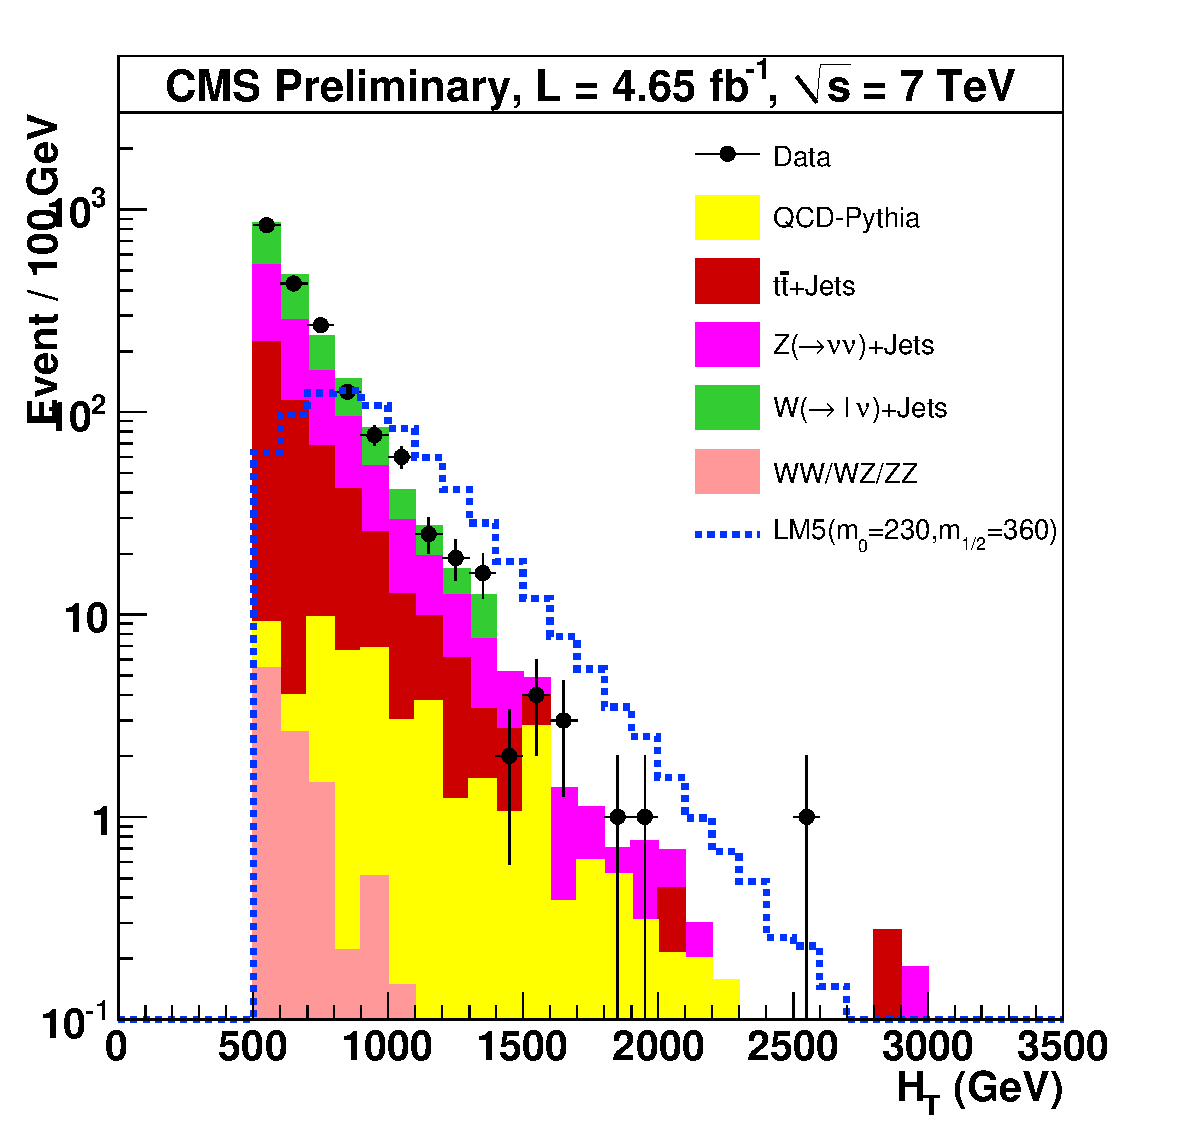
\includegraphics[width=0.5\textwidth]{figures/RA2/c_RA2_HTMHT_3J_dPhi_lepVeto_h_HT.pdf} &
      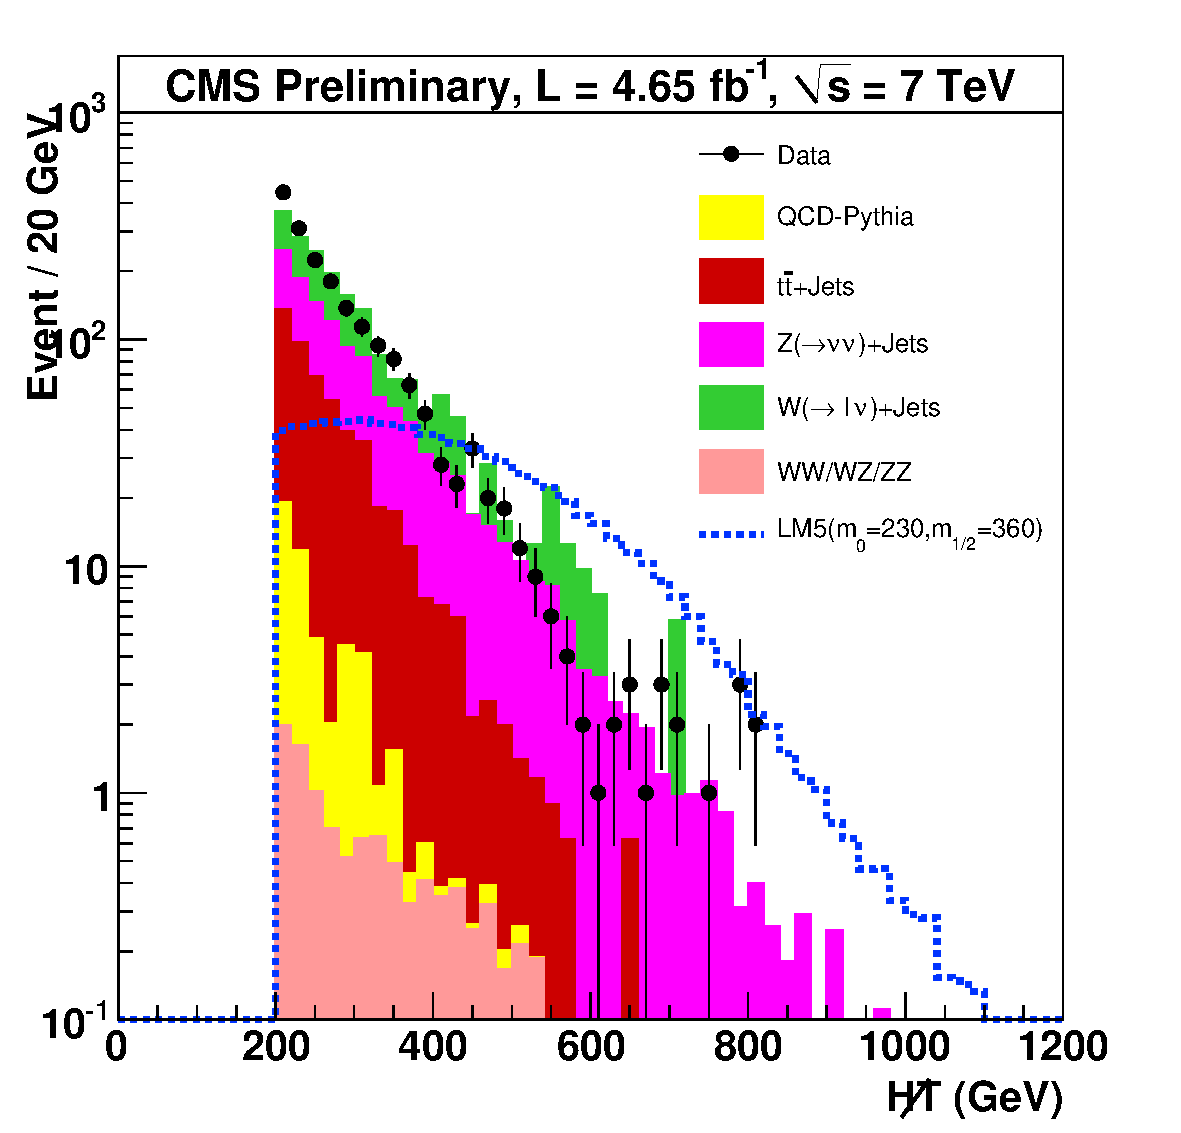
\includegraphics[width=0.5\textwidth]{figures/RA2/c_RA2_HTMHT_3J_dPhi_lepVeto_h_MHT.pdf} &
      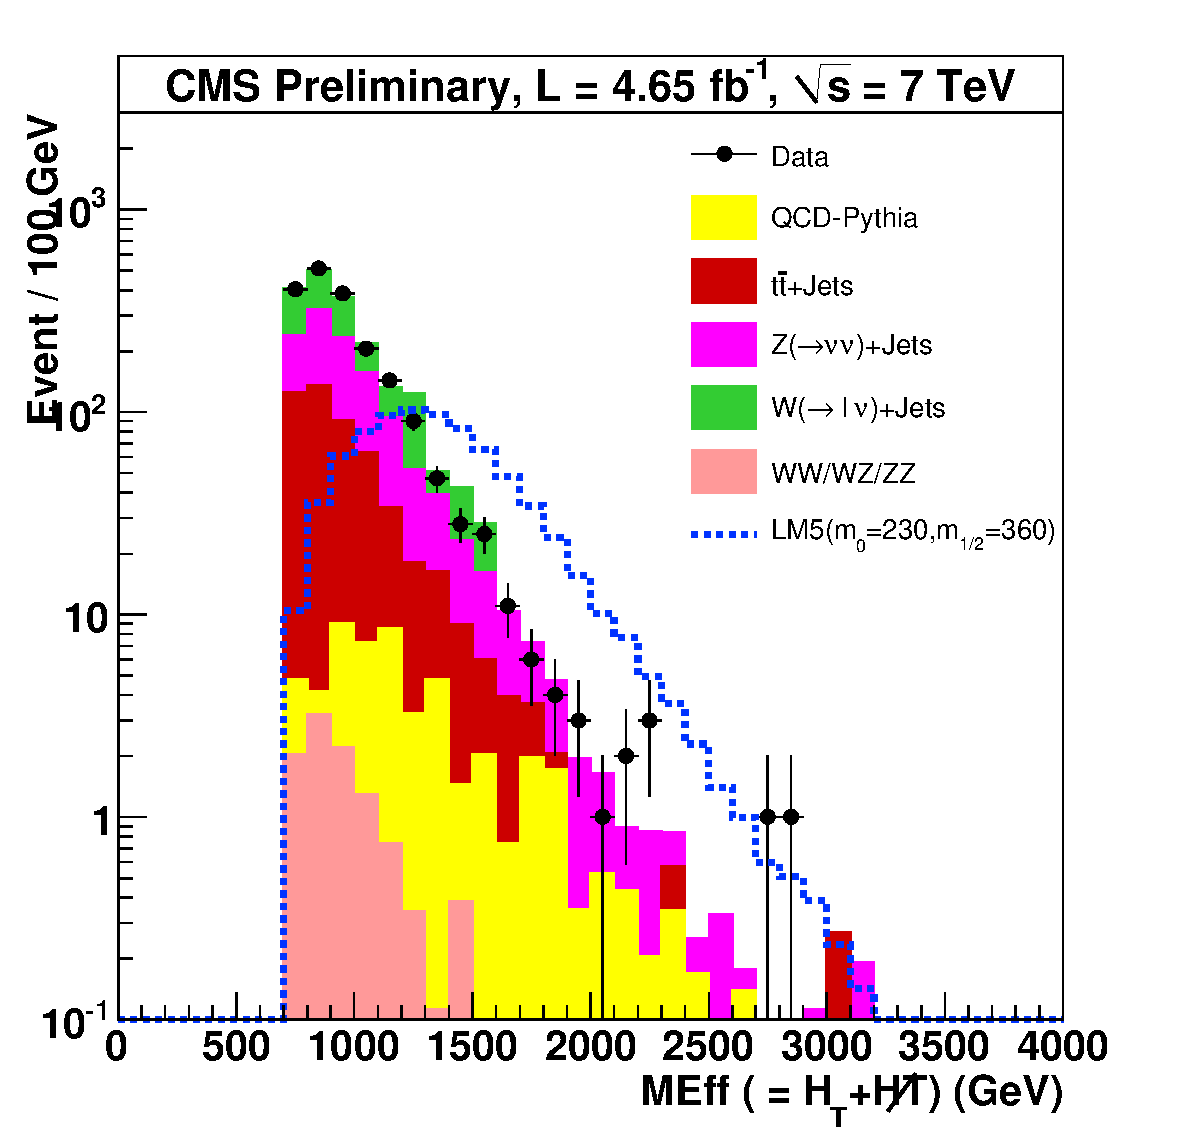
\includegraphics[width=0.5\textwidth]{figures/RA2/c_RA2_HTMHT_3J_dPhi_lepVeto_h_MEff.pdf} \\ 
    \end{tabular}
  \end{center}
  \caption{\todo{Add caption, point out difference to proper combination}}
  \label{fig:RA2:Results:Prediction}
\end{figure}




%%As outlined before in \qsec{sec:Theory:SUSY}, \susy is a promising and one of the most extensively studied frameworks for physics beyond the \sm.
%%Hence, \susy often serves as a guideline in the design of new-physics searches at collider experiments.
%%At the \lhc, sparticles can be produced, in particular squarks and gluinos via the strong interaction in the initial $pp$ collisions.
%%Due to their high masses, they subsequently decay in cascades into \sm particles with large momenta.
%%Again, since the sparticles are expected to be coloured, they will predominantly decay into coloured \sm particles and hence result in jets in the detector.
%%In case R-parity is conserved, the sparticles will be created in pairs and the LSP will be stable.
%%If only weakly interacting, such as the neutralino in the \mssm, the LSP will not produce any direct signal in the detector but will manifest as an imbalance in the observed total transverse momentum (\emph{missing transverse momentum} `\met') in the event.
%%
%%Since, of course, it is not known what kind of new physics --- if at all --- is realised at the \tevnospace scale, it is not clear either what kind of signature exactly to expect at the \lhc experiments.
%%The \cms \susy group therefore conducts a variety of searches for new physics covering a broad range of possible signatures which are motivated but not limited to supersymmetric models~\cite{bib:CMS:PhysicsResultsSUS}.
%%They can be roughly categorised as searches in lepton, photon, or multijet final states, each time accompanied by \met.
%%Each channel is covered by several analyses with different techniques and focus, thus allowing for mutual cross checks and lowering the model dependence.
%%
%%The multijet (\emph{all-hadronic}) final state is characterised by several high-\pt jets, large \met, and no isolated leptons.
%%Given the strong production mechanism and the consequent decay modes \addref, this channel has the largest branching ratio and can reach highest sensitivity.
%%At the same time however, it faces a huge background from \sm processes with the same signature, where \met is caused by neutrinos or instrumental effects.
%%%At the same time however, it faces a huge background from \sm processes with the same signature, such as \ZInvJets events as well as \ttbar and \WJets events, where the $W$ bosons either decay into light leptons which are not identified or into hadronically decaying \ltau leptons.
%%%In these cases, genuine \met is caused by neutrinos.
%%%A different major background arises from QCD multijet events where one or more jets are severely mismeasured because of leptonically decaying heavy-flavour hadrons inside the jet or because of instrumental effects.
%%
%%The presented analysis, in the following termed \emph{jets+met} analysis, has been designed as an inclusive search for new physics with minimal kinematic biases induced by the event selection in order to provide a high acceptance for a wide range of possible new physics scenarios with all-hadronic final states.
%%Therefore, the central observables in the analysis are \HT, the scalar sum of the jet transverse momenta, and \MHT, the missing transverse momentum computed from the jet momenta.
%%The broad acceptance requires a particularly precise understanding of the involved \sm backgrounds.
%%Hence, the essential feature of this analysis are robust methods to measure the full background spectra directly from data with minimal reliance on simulation.
%%The analysis has been initially published based on the 36\pbinv of data acquired by \cms in 2010~\cite{springerlink:10.1007/JHEP08(2011)155}.
%%This thesis focuses on an update which was performed with \lumiratwo from the 2011 data~\cite{CMS-PAS-SUS-11-004}.
%%
%%\cms has performed further searches in the all-hadronic channel complementing the \ratwo analysis~\cite{PhysRevLett.107.221804,bib:MT2_2011,CMS-PAS-SUS-11-008}.
%%These analyses are typically based on the assumption of initial pair-production of heavy particles and its implications.
%%Hence, different kinematic variables such as \alphat~\cite{PhysRevLett.101.221803}, $M_{\text{T},2}$~\cite{Lester:1999tx,Barr:2003rg}, or the `razor' variables $R$ and $M_{R}$~\cite{Rogan:2010kb} are exploited in order to reduce the \sm backgrounds, in particular QCD.
%%The ATLAS collaboration also published results from searches for new physics in similar all-hadronic final states\addref.
%%
%%This Chapter is organised as follows.
%%In \qsec{sec:RA2:EvtSel}, the selection of a general data set is described, from which later on more confined sets are defined in order to search for deviations from the expected \sm backgrounds.
%%The measurement of the latter from data is discussed in \qsec{sec:RA2:BkgEstimation}. 
%%Special emphasis is put on the QCD background, because the resolution measurements presented in \qsecs{sec:ResCore}{sec:ResTails} are an essential input.
%%Finally, in \qsec{sec:RA2:Results}, the results are interpreted.
%%
%%
%%(\todo{to introduction} Therefore, the investigated signatures in the search for new physics presented in this thesis have been motivated by the expectations from certain \susy scenarios.
%%However, it should be stressed, that the search has been designed in a most generic way and is sensitive to many possible realisations of physics beyond the \sm.)
%%
%%
%%
%%\section{Sample and Event Selection} \label{sec:RA2:EvtSel}
%%The presented analysis was performed on data from $pp$ collisions at a centre-of-mass energy of 7\tev which were acquired from March to June 2011 by the CMS experiment.
%%With all subdetectors fully functional, an integrated luminosity of \lumiratwo was recorded.
%%Events were collected by triggering on $\HT^{\text{trigger}}$ and, for most of the data, at the same time on $\MHT^{\text{trigger}}$, where $\HT^{\text{trigger}}$ and $\MHT^{\text{trigger}}$ are computed from calorimeter jets clustered with the iterative-cone algorithm with cone size $0.5$.
%%The efficiency of the combined set of triggers has been measured in data using a more inclusive  $\HT^{\text{trigger}}$ trigger as a function of the offline \HT and \MHT defined below in \qsec{}:
%%it is greater than $99\%$ for \mbox{$\HT > 350\gev$} and \mbox{$\MHT > 200\gev$}~\cite{CMS-PAS-SUS-11-004}.
%%
%%All offline physics objects have been reconstructed with the \emph{particle-flow} (`\PF') algorithm~\cite{CMS-PAS-PFT-09-001,CMS-PAS-PFT-10-002}.
%%For this procedure, the information from all CMS subdetectors are combined to identify different types of particles, such as charged or neutral hadrons, photons, muons, and electrons.
%%From these particles, jets are clustered using the \antikt jet algorithm~\cite{1126-6708-2008-04-063} with a distance parameter \mbox{$R=0.5$}.
%%Their momenta are corrected on average by removing the $\eta$ and \pt dependence as well as by compensating for the impact of additional pile-up interactions to those which would have been obtained if all particles were perfectly measured.
%%The calibration constants were derived from simulation.
%%%They are corrected with calibration constants derived from simulation in order to remove the $\eta$ and \pt dependence of their energy scale as well as to compensate for the impact of additional pile-up interactions.
%%Residual small response differences between data and simulation are corrected by applying additional calibration constants to the data, which are measured from photon+jets and dijet data~\cite{1748-0221-6-11-P11002}.
%%\todo{Explain this in more detail in the jet section.}
%%
%%Several \emph{filters} have been employed in order to identify events where the object reconstruction failed or was spoiled by instrumental effects or which originated in beam-background processes.
%%In rare cases, these events feature large \MHT and can populate the search regions.
%%Although their absolute contribution is small \todo{put some number}, they might substantially falsify the analysis result due to the likewise tiny expected rate of signal processes.
%%Therefore, these events are not used in the further analysis.
%%\addfig{effect of cleaning (note by Colin, new 2011 results)}
%%
%%Particles originating from displaced vertices in satellite collisions as well as from beam-related processes such as muons from proton collisions outside the detector (\emph{beam halo}) possibly prevent a proper event reconstruction.
%%Therefore, each event is required to have at least one high-quality primary vertex which has been determined from more than four tracks and is located within $24\cm$ in $z$ and $2\cm$ in $xy$ direction from the nominal interaction point.
%%Furthermore, the \emph{Cathode Strip Chamber} subdetector is utilised to identify and reject events with muons traversing parallel to the beam and hence likely stem from a beam halo~\cite{CMS-PAS-MUO-10-002}.
%%
%%In some events, anomalous signals in the electromagnetic or hadronic calorimeters are caused by particles hitting the readout electronics, scintillation fibres, or photomultipliers.
%%Dedicated criteria have been defined to identify and reject these events~\cite{CMS-PAS-EGM-10-006,CMS-DP-2010-025}.
%%Faked large energy deposits are in rare cases also produced by electronic noise in the ECAL readout system at random times and can overlap with a collision event.
%%These anomalies can be identified and in fact removed using timing and pulse-shape information, thus allowing further usage of the event~\cite{CMS-PAS-JME-10-009}.
%%%Additional rare noise has been identified to affect the ECAL endcaps coherently with the muons systems.
%%%It has been suppressed by selecting events with less than $2\,500$ energy deposits in the endcaps (\emph{EE noise filter}).
%%
%%Reliable track reconstruction is ensured by requiring the fraction of tracks passing high-quality criteria to be greater than $25\%$, if there are at least ten tracks in the event.
%%In addition, the scalar sum of the \pt of tracks associated to the primary vertex has been required to be less than $10\%$ of the scalar sum of jet \pt of all jets within the tracker acceptance in order to ensure.
%%Moreover, events with seriously misreconstructed muons are rejected~\cite{springerlink:10.1007/JHEP08(2011)155,CMS-PAS-SUS-11-004}.
%%
%%About $1\%$ of the crystals of the electromagnetic calorimeter are not read out because of malfunctioning on-detector electronics.
%%If energy is deposited in these crystals, it is lost in the object reconstruction.
%%The affected events are identified and rejected either by the information from a parallel readout chain of the trigger system or, in case it is not available, by measuring the amount of energy deposited in the crystals surrounding the affected regions~\cite{CMS-PAS-JME-10-009}.
%%
%%After the trigger and filter requirements, the full event selection is defined as follows in two succesive steps starting with the (\emph{baseline selection}):
%%\begin{itemize}
%%\item There are at least three jets with \mbox{$\pt > 50\gev$} and $|\eta| < 2.5$ in order to select events with a multijet final state topology.
%%\item A high energy scale of the hard-scattering process is ensured by requiring \mbox{$\HT > 350\gev$}, where
%%  \begin{equation*}
%%    \HT \equiv \sum_{i} \pti{i}
%%  \end{equation*}
%%  and $i$ runs through all jets with \mbox{$\pt > 50\gev$} and \mbox{$|\eta| < 2.5$}.
%%\item In order to suppress QCD contributions, \mbox{$\MHT > 200\gev$} has to be met, where
%%  \begin{equation*}
%%    \MHT \equiv -\left|\sum_{i} \ptivec{i} \right|
%%  \end{equation*}
%%  and $i$ runs through all jets with \mbox{$\pt > 30\gev$} and \mbox{$|\eta| < 5$} \todo{motivate choice of different jets in \HT and \MHT}.
%%\item Remaining QCD events in which large \MHT is caused by a single mismeasured jet are vetoed by requiring \mbox{$\Delta\phi(\ptivec{i},\MHTvec) > 0.5$}, \mbox{$i\in{1,2}$}, and \mbox{$\Delta\phi(\ptivec{3},\MHTvec) > 0.3$}, \ie \MHT must not be aligned with the transverse momenta of one of the leading three jets.
%%\item \ttbar and \WJets events with leptons in the final state are suppressed by rejecting events containing isolated muons or electrons with \mbox{$\pt > 10\gev$} and \mbox{$|\eta| < 2.4$} or \mbox{$|\eta| < 2.5$}, respectively~\cite{CMS-PAS-SUS-11-004}.
%%\end{itemize}
%%Three \emph{search regions} are defined by tighter criteria on \HT and \MHT \wrt the baseline selection.
%%They are selected based on the amount of \sm background and the expected signal efficiency for the \cmssm:
%%\begin{itemize}
%%\item The \emph{medium search region} requires \mbox{$\HT > 500$} and \mbox{$\MHT > 350\gev$}.
%%\item The \emph{high-\HT search region} requires \mbox{$\HT > 800\gev$}.
%%This selection is in particular sensitive to events with high multiplicities as in case of long cascade decays where most of the energy is distributed to the strongly interacting particles.
%%\item The \emph{high-\MHT search region} requires \mbox{$\MHT > 500\gev$} in order to improve the rejection of \sm backgrounds, especially QCD.
%%\end{itemize}
%%The expected total event yields\footnote{The simulated yields for the individual background contributions are quoted in Tab.~1 in~\cite{CMS-PAS-SUS-11-004}.} from the \sm background processes as obtained from simulation after the baseline and three search selections are listed in \qtab{tab:RA2:EventSel:EventYields}.
%%They are compared to the expectations for a specific \susy model.
%%\begin{table}[!htb]
%%  \begin{center}
%%    \caption{Number of events expected from the \sm background processes in \lumiratwo after the baseline and search selections as predicted by simulation.
%%      The contributions have been obtained using the \pythia generator in case of QCD and the \madgraph generator otherwise.
%%      For comparison, the expected number of signal events for the \cmssm parameter point `LM4', defined by \mbox{$m_{0} = 210\gev$}, \mbox{$m_{1/2} = 285\gev$}, \mbox{$A_{0} = 0$}, \mbox{$\tan\beta = 10$}, and \mbox{$\mu > 0$}, is given to illustrate the impact from possible new physics.
%%      The events have been generated using \pythia assuming a next-to-leading order LM4 signal cross section of \mbox{$2.5\;\text{pb}$}, which has been computed using the \prospino programme~\cite{Beenakker:1996ed}.
%%    }
%%    \label{tab:RA2:EventSel:EventYields}
%%    \begin{tabular}{l r@{.}l r@{.}l r@{.}l r@{.}l}
%%      \toprule
%%      & \multicolumn{2}{c}{Baseline} & \multicolumn{2}{c}{Medium} & \multicolumn{2}{c}{High-\HT} & \multicolumn{2}{c}{High-\MHT} \\
%%      & \multicolumn{2}{c}{(\HT$>$350~\gev)}  & \multicolumn{2}{c}{(\HT$>$500~\gev)} & \multicolumn{2}{c}{(\HT$>$800~\gev)}  & \multicolumn{2}{c}{(\HT$>$800~\gev)}  \\
%%      & \multicolumn{2}{c}{(\MHT$>$200~\gev)} & \multicolumn{2}{c}{(\MHT$>$350~\gev)} & \multicolumn{2}{c}{(\MHT$>$200~\gev)} & \multicolumn{2}{c}{(\MHT$>$500~\gev)} \\
%%      \midrule
%%      \sm
%%      & 987&0 
%%      &  95&0 
%%      &  83&0 
%%      &   7&5  \\
%%      \midrule
%%      LM4
%%      & 742&0 
%%      & 318&0 
%%      & 304&0 
%%      &  54&0  \\
%%      \bottomrule
%%    \end{tabular}
%%  \end{center}
%%\end{table}
%%
%%
%%
%%\section{Estimation of the Standard Model Backgrounds From Data} \label{sec:RA2:BkgEstimation}
%%Several \sm processes with genuine \met caused by neutrinos constitute backgrounds to the selected signal samples.
%%These are \ZInvJets events as well as \ttbar and \WJets events, where the $W$ bosons either decay into light leptons which are not identified or into hadronically decaying \ltau leptons.
%%A different major background arises from QCD multijet events where one or more jets are severely mismeasured because of leptonically decaying heavy-flavour hadrons inside the jet or because of instrumental effects.
%%The expected, full \HT and \MHT spectra of the \sm background processes are modelled from data, as discussed below, thus avoiding dependence on the simulation.
%%
%%
%%
%%\subsection{Non-QCD Backgrounds}
%%% --- Z to inv bkg ------------------------------------
%%Events with jets and a \Z boson produced in association which subsequently decays into two neutrinos form an irreducible \sm background in the selected data sample.
%%
%%Its contribution can be estimated from data in a straightforward way using \mbox{$Z\rightarrow e^{+}e^{-}$}+jets or \mbox{$Z\rightarrow \mu^{+}\mu^{-}$}+jets events and ignoring the leptons in the reconstruction in order to mimic the neutrino-induced \MHT in \ZInvJets events.
%%After corrections for the acceptance, efficiency, and different branching ratios, their topology is directly reproduced due to the lepton-universality of the weak interaction and the expected background yield is obtained by applying the jet-related selection criteria.
%%However, given the low yield of the \mbox{$Z\rightarrow ll$}+jets events, this method is used as a cross-check verifying the results of the primary method.
%%
%%As primary method, the kinematic properties of \ZInvJets events are predicted from a control sample of $\gamma$+jets events.
%%The structure of the production process is the same for the neutral electro-weak bosons at \pt larger than the \Z mass with asymptotically vanishing mass effects and the cross-section ratio depends mostly on the different size of the electro-weak couplings.
%%In order to obtain a reliable background prediction, contributions to the control sample from QCD multijet events where a photon originates not in the hard scattering process but in fragmentation inside jets or neutral pion decays are minimised by imposing tight isolation criteria on the reconstructed photons.
%%The residual contamination is estimated from NLO \textsc{Jetphox} calculations and data, respectively~\cite{PhysRevD.73.094007,PhysRevLett.106.082001,PhysRevD.84.052011}\todo{verify}.
%%The selection requirements have also been found to sufficiently suppress contamination of the control sample by possible signal events.
%%Then, the background prediction is obtained by removing the $\gamma$ in the event reconstruction, applying the jet-related selection requirements to the control sample, and finally scaling the resulting number of $\gamma$+jets events to account for the differences in branching ratios as well as acceptance and reconstruction efficiencies, which are determined from a \madgraph simulation~\cite{Alwall:2007st}.
%%The dominant uncertainties of the method are an uncertainty of $12\%$ on this phenomenological scale factor as well the statistical uncertainty of about $15\%$ due to the size of the control sample.
%%
%%
%%% --- Lost-lepton and hadronic tau bkg ---------------------------------
%%Events from \ttbar and \WJets production can fake the signal topology if the $W$ bosons decay into leptons and neutrinos thus inducing \met.
%%They are not rejected by the event selection either in case of a hadronically decaying \ltau lepton (\emph{hadronic-$\tau$}) or in case the veto of a light lepton fails (\emph{lost-lepton}) because it is out of geometric or kinematic acceptance, is not identified, or not isolated.
%%Both components are predicted using a $\mu$+jets control sample.
%%
%%In case of the \lostlep background, control samples for the different search regions are selected by applying the full event selection but without the explicit lepton veto.
%%Instead, exactly one well-identified and well-isolated muon is required.
%%Moreover, only events with a \emph{transverse mass} \mbox{$m_{\text{T}}\equiv\sqrt{2\pt(\mu)\met(1-\cos(\Delta\phi))}$} of less than 100\gev are selected, with $\Delta\phi$ being the difference in azimuthal angle between the muon and the \met vector, which enhances the \ttbar and \WJets contributions in the sample and sufficiently suppresses the presence of possible signal events.
%%The \lostlep contribution in the search regions is modelled by weighting the number of events in the control sample according to the lepton identification and isolation efficiencies as well as acceptance factors.
%%The identification and isolation efficiencies are measured separately for electrons and muons from $Z$+jets data as a function of lepton \pt using a tag-and-probe method.
%%They are parametrised by the angular distance between the lepton and the nearest jet as well as the lepton $\eta$, respectively, in order to take into account kinematic differences of the $Z$+jets events.
%%Residual kinematic differences have been studied using simulated events and have been found to result in an underprediction of the background of about $7\%$, for which the final prediction has been corrected.
%%The acceptance factor is determined from simulated \ttbar and \WJets events.
%%Besides the correction of the kinematic bias, the dominant uncertainty of the prediction arises from the statistical uncertainty of $22\%$ due to the size of the $\mu$+jets and $Z$+jets control samples.
%%
%%In case of the \hadtau background, the control sample is selected using a single-muon trigger and requiring exactly one muon with \mbox{$\pt > 20\gev$} and \mbox{$|\eta| < 2.1$}.
%%Again, the transverse mass requirement is imposed to prevent signal contamination of the control sample.
%%Due to the lepton universality of the weak interaction, the hadronic part of the events in the control sample correspond to the non-$\tau$ part of the \hadtau background events.
%%Hence, the muon is used to model the $\tau$ jet by scaling its transverse momentum with a factor sampled from a template of the visible $\tau$-\pt fraction, which has been obtained from simulated events.
%%After recomputation of \HT and \MHT, where the additional jet is taken into account, the \hadtau contribution in the search region is predicted by applying the search selection to the modified control sample and scaling the event yield by the branching fraction of $W$ bosons decaying into hadronically decaying $\tau$ leptons and into muons.
%%Corrections are applied to take into account the muon geometric and kinematic acceptance, which is derived from simulation, as well as the identification and isolation efficiencies, which are measured from $Z$+jets data as in case of the \lostlep background.
%%The dominant uncertainties of the prediction are the uncertainty on the $\tau$-\pt template and the statistical uncertainty due to the size of the control sample, each amounting to about $3\%$.
%%
%%
%%\subsection{QCD Background}
%%\todo{discuss jet response, mc scaling} \\
%%\todo{discussion: where does qcd contribute (high ht search region, i.e. high m1/2)}
%%
%%Modelling of the QCD multijet background is challenging because the underlying QCD production processes are theoretically difficult to compute and the simulation of jet measurements requires a particularly precise understanding of the detector components and effects. 
%%In QCD multijet events, \MHT arises from mismeasurements due to the jet-\pt response \alreadydefined{response}.
%%While the almost Gaussian core of the response distribution around unity is inherent to the principle of energy and momentum measurement of a detector, the tails of extremely low response originate both in heavy-flavour hadrons inside jets which decay into among others neutrinos and in instrumental effects such as punch-through of energetic particles as well as masked detector regions.
%%\todo{add study here or elsewhere of response components (Sue Ann)}
%%Although the tail component contributes only below the percentage level to the total distribution, it leads to severe jet-\pt mismeasurements resulting in possibly large values of \MHT and thus promoting an event into the search regions.
%%
%%\subsubsection{Description of the Rebalance-And-Smear Method}
%%The QCD background is estimated from inclusive multijet data using a simplified simulation obtained by a \emph{rebalance-and-smear} (`R+S') method~\cite{bib:phd:sueann,CMS-PAS-SUS-11-004,springerlink:10.1007/JHEP08(2011)155}.
%%An estimator of \MHT is obtained by first rebalancing the jet momenta in each event, taking into account the jet-\pt resolution, and then weighting the rebalanced momenta by the full jet-\pt response distribution in order to predict the complete multijet kinematics.
%%
%%In the rebalance step, a sample of \emph{seed events} is created from multijet data.
%%The measured jet momenta are adjusted, resulting in \emph{seed jets}, to regain approximate transverse momentum balance as expected for QCD events at particle-jet level.
%%Technically, this is achieved with a kinematic fit~\addref.
%%\pt, $\eta$, and $\phi$ of the jets are varied in order to find a configuration which obeys the transverse momentum balance constraint and minimises the residuals of measured and modified jets.
%%The measurement uncertainties are approximated by the Gaussian core component of the jet-\pt response distribution since the rebalance procedure is insensitive to the tiny non-Gaussian tails.
%%Only jets with \mbox{$\pt > 10\gev$} are used in order to reduce the impact of pile-up interactions, which produce a large number of low-\pt jets not originating in the considered hard interaction and thus spoiling the momentum balance constraint.
%%Possible biases introduced by this requirement have been observed to affect the final prediction by less than $10\%$ and are considered in the uncertainties.
%%Importantly, contributions to the seed sample from the \ttbar or electro-weak backgrounds as well as possible signal processes are negligible since also these events will be transformed into QCD-like events with balanced transverse momenta and their cross section is smaller by orders of magnitude than the QCD-multijet cross-section.
%%
%%In the smear step, the four-momentum of each seed jet is scaled by a random factor generated from the full jet-\pt response distribution, thus modelling effects of the measurement and resulting in the expected detector-level jet.
%%The kinematic of the original QCD events is preserved in the obtained sample of events with smeared jets.
%%Hence, the expected distributions of \HT and \MHT as well as other jet-related variables are predicted after applying the full analysis event selection.
%%In order to improve the statistical precision of the prediction, the smear step of the procedure is repeated 1000 times for each seed event.
%%Biases due to the correlated seeds are avoided by incorporation of a bootstrap technique~\cite{bib:bootstrap} when computing the mean and variance of the prediction.
%%
%%The performance of the R+S method has been studied using a sample of events simulated with \pythia.
%%The predicted \HT and \MHT distributions after a modified baseline selection, where the \HT and \MHT requirement has been dropped, respectively, are shown in \qfig{fig:RA2:SMBkg:RSClosure}.
%%They are compared to the distributions from the fully simulated events.
%%There is good agreement of the R+S prediction to the full simulation in the important medium-to-high \MHT region, except for the highest bin where the number of events are seriously overpredicted; the precise amount is difficult to quanitfy, however, since the statistical uncertaintiy of the expectation from the full simulation is large.
%%In the low \MHT region, the prediction fluctuates around the expectation by up to $20\%$, which is not covered by the statistical uncertainties.
%%The ratio of the predicted number of events to the number obtained with the full simulation for the different search selections is applied as a bias correction factor to the final prediction.
%%It is below $25\%$ in all cases.
%%The dominating biases of the method arise from the finite jet-\pt response parametrisation, the jet-\pt threshold of 10\gev for the rebalance step, and from migration effects due to the steeply falling jet-\pt spectrum in combination with the finite resolution.
%%\begin{figure}
%%  \begin{center}
%%    \begin{tabular}{cc}
%%%      \includegraphics[width=0.5\textwidth]{figures/ra2/} &
%%      & \includegraphics[width=0.5\textwidth]{figures/ra2/QCD_SmearingClosure_OnMC_LowHT_MHT.pdf} \\
%%    \end{tabular}
%%  \end{center}
%%  \caption{\fixme{Add HT distribution} Consistency test of the R+S method with \pythia-simulated events~\cite{CMS-PAS-SUS-11-004}: \HT (\textit{left}) and \MHT (\textit{right}) distributions predicted by the R+S method (circles) compared to the results of the full simulation (squares).
%%  }
%%  \label{fig:RA2:SMBkg:RSClosure}
%%\end{figure}
%%
%%
%%
%%\subsubsection{Jet Response Functions}
%%The jet-\pt response distributions are crucial input to the R+S method.
%%They are determined as described in \qsec{sec:Jets:Resolution:MCTruth} from a sample of QCD multijet events simulated with the \pythia event generator~\cite{Sjostrand:2006za}: to each of the two leading \todo{define leading at first appearance} generator-level jets the reco-level jet closest in \mbox{$\eta\times\phi$} is matched, and the response is computed as \mbox{$\ptreco / \ptgen$}.
%%The simulated distributions are adjusted to match the data as discussed in detail in \qsec{}.
%%In order to account for the dependence of the response on the energy of the jet as well as the different detector region, a set of response distributions for different bins of \pt and $|\eta|$ is compiled.
%%
%%
%%\subsubsection{Prediction of the QCD Background}
%%In contrast to the search sample, the multijet data input to the R+S method has been collected by triggering on $\HT^{\text{trigger}}$ only with no additional requirement on \MHT, which would bias the seed sample.
%%However, the lowest un-prescaled \HT trigger has a threshold of 500\gev.
%%Since the baseline selection requires \mbox{$\HT > 350\gev$} and since in course of the R+S procedure events can migrate in \HT, additional, prescaled trigger paths with thresholds down to 150\gev are utilised.
%%The data sample recorded by the different trigger paths are combined taking into account the prescales, which results in an increase of the statistical uncertainty of the prediction of about \todo{add number} because of single events with large weights.
%%Furthermore, to reduce the amount of processed data, only events containing at least two jets with \mbox{$\pt > 50\gev$} are considered for the seed sample.
%%The results of the R+S prediction in the different search regions are listed in \qtab{tab:RA2:Bkg:RS}.
%%\begin{table}[!htb]  
%%  \begin{center}
%%    \caption{\todo{Add caption}}\label{tab:RA2:Bkg:RS}
%%    \begin{tabular}{lllll}
%%      \toprule
%%      & Baseline & Medium & High-\HT & High-\MHT \\
%%      \midrule
%%      Bias-corrected prediction & 31.0 & 1.3 & 13.5 & 0.09 \\
%%      Total uncertainty ($\%$) & $^{+125}_{-116}$ & $^{+112}_{-107}$ & $^{+62}_{-44}$ & $^{+347}_{-345}$ \\
%%      \midrule
%%      Seed sample size ($\%$) & $\pm114$ & $\pm102$ & $\pm30$ & $\pm340$ \\
%%      Resolution core ($\%$) & $^{+10}_{-8}$ & $^{+3}_{-8}$ & $^{+9}_{-9}$ & $^{+1}_{-18}$\\
%%      Resolution tail ($\%$) & $^{+31}_{-19}$ & $^{+17}_{-34}$ & $^{+33}_{-31}$ & $^{+41}_{-36}$\\
%%      Flavour trend ($\%$) & $\pm10$ & $\pm10$ & $\pm10$ & $\pm10$\\
%%      R+S non-closure ($\%$) & $\pm40$ & $\pm40$ & $\pm40$ & $\pm40$\\
%%      Pile-up effects ($\%$) & $\pm10$ & $\pm10$ & $\pm10$ & $\pm10$\\
%%      \bottomrule
%%    \end{tabular}
%%  \end{center}
%%\end{table}
%%
%%
%%\subsubsection{Systematic Uncertainties}
%%Various sources of systematic uncertainties of the R+S method have been investigated.
%%Their impact on the prediction is also listed in~\qtab{tab:RA2:Bkg:RS}.
%%
%%As discussed above, the combined impact of the R+S biases has been found to affect the prediction by less than $25\%$ depending on the search region.
%%The final prediction is corrected for this bias and a conservative systematic uncertainty of $40\%$ is assigned.
%%
%%Furthermore, the uncertainties on the jet-\pt response measurements~\qsec{} are propagated to the prediction by repeating the R+S method with the response input changed by \mbox{$\pm1\sigma$}, leading to variations of the result of up to $40\%$.
%%
%%The simulated response distributions were derived using the \pythia event generator.
%%Variations of the R+S prediction due to the assumed flavour composition of jets were observed to be within $10\%$ when comparing to the results obtained with response distributions from the \madgraph generator~\cite{bib:phd:sueann,CMS-PAS-SUS-11-004,springerlink:10.1007/JHEP08(2011)155}.
%%
%%Residual effects from pile-up interactions have been investigated using a sample of simulated events, where the pile-up scenario has been reweighted to match the distribution expected for data from the machine conditions and the minimum-bias cross section.
%%No significant variations in the R+S prediction are present when shifting the mean of the pile-up distribution by \mbox{$\pm1$}.
%%Nonetheless, given the sizable statistical uncertainties of the different results, a conservative uncertainty of $10\%$ is assigned.
%%
%%
%%
%%\section{Results and Interpretation} \label{sec:RA2:Results}
%%The \HT and \MHT distributions in \lumiratwo of data after the baseline selection are shown in \qfig{fig:RA2:Results:HTMHT}.
%%They are compared to the expected \sm background contributions predicted using the data-driven methods described above.
%%\begin{figure}
%%  \begin{center}
%%    \begin{tabular}{cc}
%%      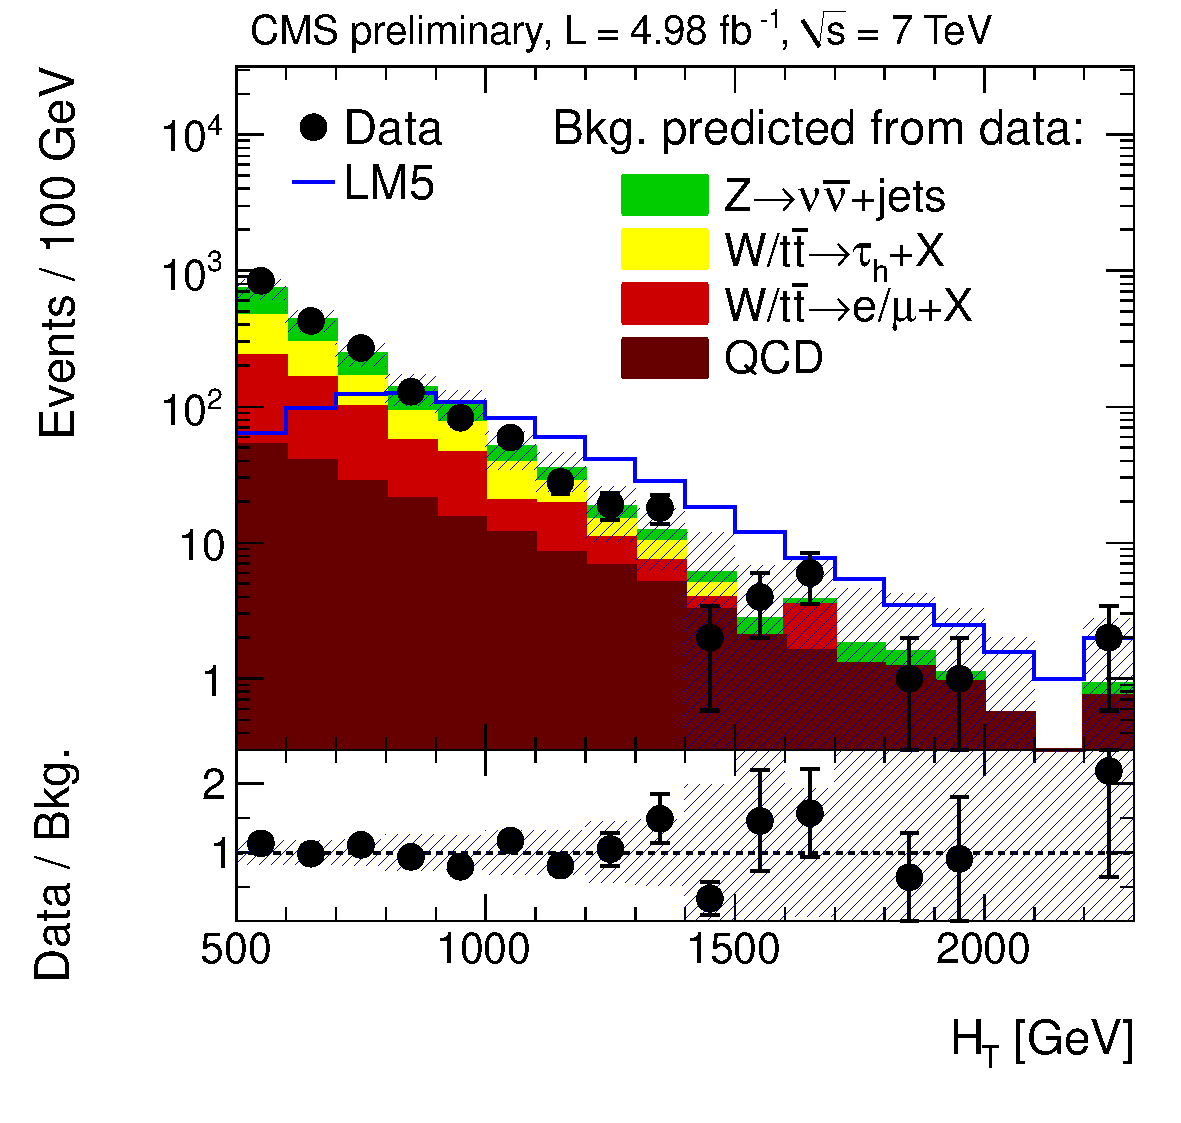
\includegraphics[width=0.5\textwidth]{figures/ra2/RA2DataVsEstimatedBkg_HT.pdf} &
%%      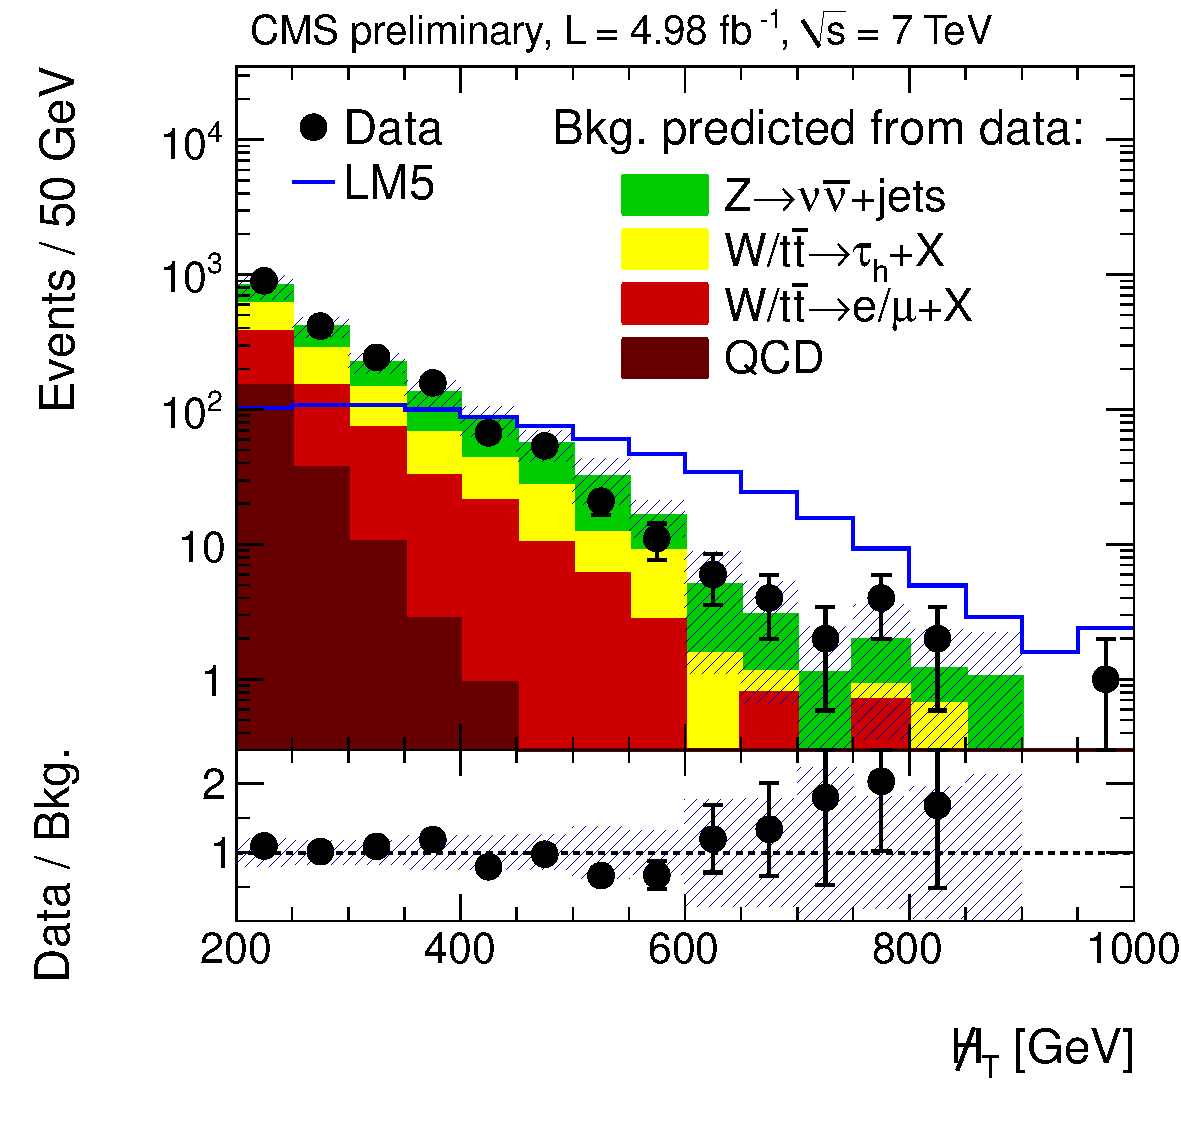
\includegraphics[width=0.5\textwidth]{figures/ra2/RA2DataVsEstimatedBkg_MHT.pdf} \\
%%    \end{tabular}
%%  \end{center}
%%  \caption{\todo{Add caption, point out difference to proper combination}}
%%  \label{fig:RA2:Results:HTMHT}
%%\end{figure}
%%
%%The number of events observed in data after the baseline and the different search selections is listed in \qtab{tab:RA2:Results:EventYields}.
%%It is compared to the yields expected from the different \sm background processes.
%%Although the data-driven methods allow for a prediction differential in \HT and \MHT, here integrated yields in the more inclusive search regions are considered in order to achieve maximal statistical precision.
%%A combined background expectation is derived by numerical convolution of the different probability density functions assigned to each uncertainty source of the individual background contributions, thus taking into account possible correlations between the estimation methods.
%%Following the Central Limit Theorem, the resulting probability density distribution is fitted with a Gaussian function, whose mean and standard deviation are listed as total expected background yield and its uncertainty, respectively.
%%It is below the \sm expectation obtained from simulation listed in \qtab{tab:RA2:EventSel:EventYields}, which emphasises the importance of simulation-independent, data-driven methods.
%%The observed number of events is compatible with the \sm expectation in all search regions.
%%\begin{table}[!htb]
%%  \begin{center}
%%    \caption{Expected event yields with statistical and systematic uncertainties, respectively, from the different \sm background processes in \lumiratwo as predicted by the data-driven methods after the baseline and search selections.
%%      The total background estimate is calculated as described in the text as mean of a Gaussian fit to the combined probability density of the various uncertainty contributions.
%%      It is compared to the observed number of events in data.
%%    }
%%    \label{tab:RA2:Results:EventYields}
%%    \begin{tabular}{l
%% r@{.}l@{$\;\pm\,$}r@{.}l@{$\;^{+}_{-}$}l
%% r@{.}l@{$\;\pm\,$}r@{.}l@{$\;^{+}_{-}$}l
%% r@{.}l@{$\;\pm\,$}r@{.}l@{$\;^{+}_{-}$}l
%% r@{.}l@{$\;\pm\,$}r@{.}l@{$\;^{+}_{-}$}l
%%}
%%      \toprule
%%      & \multicolumn{5}{c}{Baseline} & \multicolumn{5}{c}{Medium} & \multicolumn{5}{c}{High-\HT} & \multicolumn{5}{c}{High-\MHT} \\
%%      & \multicolumn{5}{c}{(\HT$>$350~\gev)}  & \multicolumn{5}{c}{(\HT$>$500~\gev)} & \multicolumn{5}{c}{(\HT$>$800~\gev)}  & \multicolumn{5}{c}{(\HT$>$800~\gev)}  \\
%%      & \multicolumn{5}{c}{(\MHT$>$200~\gev)} & \multicolumn{5}{c}{(\MHT$>$350~\gev)} & \multicolumn{5}{c}{(\MHT$>$200~\gev)} & \multicolumn{5}{c}{(\MHT$>$500~\gev)} \\
%%      \midrule
%%      \ZInv
%%      &376&3  & 12&3   & $^{79.2}_{79.2}$
%%      & 42&6  &  4&4   & $^{8.9}_{8.9}$
%%      & 24&9  &  3&5   & $^{5.2}_{5.2}$
%%      &  2&4  &  1&1   & $^{0.5}_{0.5}$  \\
%%      $\ttbar/W \rightarrow e,\mu+$X
%%      &243&5  & 19&8   & $^{30.0}_{30.9}$
%%      & 12&7  &  3&3   & $^{1.5}_{1.5}$
%%      & 22&5  &  6&7   & $^{3.0}_{3.1}$
%%      &  0&8  &  0&8   & $^{0.1}_{0.1}$  \\
%%      $\ttbar/W \rightarrow \tau_{\text{had}}+$X
%%      &263&0  &  8&0   & $^{7.4}_{7.4}$
%%      & 17&0  &  2&0   & $^{0.7}_{0.7}$
%%      & 18&0  &  2&0   & $^{0.5}_{0.5}$
%%      &  0&73 &  0&73  & $^{0.04}_{0.04}$  \\
%%      QCD
%%      & 30&9  & 35&2   & $^{16.6}_{6.2}$
%%      &  1&3  &  1&3   & $^{0.6}_{0.4}$
%%      & 13&5  &  4&1   & $^{7.3}_{4.3}$
%%      &  0&09 &  0&31  & $^{0.05}_{0.04}$  \\
%%      \midrule
%%      Total
%%      & 927&5 & 103&\multicolumn{2}{l}{\hspace{-0.21cm}1}
%%      &  73&9 &  11&\multicolumn{2}{l}{\hspace{-0.21cm}9}
%%      &  79&4 &  12&\multicolumn{2}{l}{\hspace{-0.21cm}2}
%%      &   4&6 &   1&\multicolumn{2}{l}{\hspace{-0.21cm}5} \\
%%      \midrule
%%      Observed
%%      & \multicolumn{5}{l}{986.0}
%%      & \multicolumn{5}{l}{78.0}
%%      & \multicolumn{5}{l}{70.0}
%%      & \multicolumn{5}{l}{3.0}  \\
%%      \bottomrule
%%    \end{tabular}
%%  \end{center}
%%\end{table}
%%
%%Given the absence of any signal of new physics, the results are used to constrain possible models of new physics.
%%The interpretation is performed using the \CLs method~\cite{Lyons:411537,0954-3899-28-10-313,Thomas1999435}, which was developed for the Higgs searches at LEP to derive parameter limits in case of small expected signal rates at the limit of the experimental sensitivity.
%%In order to quantify the degree of agreement between the data and a specific hypothesis, a function, the \textit{test statistic}, of the experimental observables and the parameters of the tested new-physics model is defined. 
%%Two hypotheses $x$ are considered, the \textit{background hypothesis} (`$b$') where the observations are expected to originate in \sm processes only, and the \textit{signal+background hypothesis} (`$s+b$') where additional contributions arise from the new-physics model.
%%Typically, the test-statistic is monotonically increasing with larger values implying less compatibility with the background-only hypothesis.
%%The \textit{confidence level} $\CL_{x}$ of a specific hypothesis $x$ is given by the probability to obtain a value $Q$ of the test-statistic less than or equal to the value $Q_{\text{obs}}$ actually observed in data,
%%\begin{equation*}
%%  \CL_{x} \equiv P_{x}(Q \leq Q_{\text{obs}}) \;.
%%\end{equation*}
%%In case the total number of observed events in data is small and fluctuates below the average expectation for the background-only hypothesis, the confidence level $\CL_{s+b}$ might result in unphysical estimates of the model parameters and strong exclusion limits on the signal.
%%To avoid alleged exclusion of a signal to which the experiment has no sensitivity, instead the ratio
%%\begin{equation*}
%%  \CLs \equiv \frac{\CL_{s+b}}{\CL_{b}}
%%\end{equation*}
%%is used to derive limits.
%%The signal hypothesis is defined as being excluded at the confidence level $\alpha$ if
%%\begin{equation*}
%%  1-\CLs \leq \alpha \;.
%%\end{equation*}
%%
%%Here, exclusion limits at the $95\%$ confidence level are derived on the parameters of the \cmssm.
%%The expected number of signal events in the different search regions are determined from simulated events assuming \mbox{$\tan\beta = 10$}, \mbox{$\mu > 0$}, and \mbox{$A_{0} = 0$}.
%%The values of $m_{0}$ and $m_{1/2}$ have been varied in steps of 20\gev, and for each point a sample of $10\;000$ events has been generated using the \isajet programme~\cite{bib:isajet} with the subsequent fragmentation and hadronisation processes simulated by \pythia.
%%Signal cross sections have been corrected by next-to-leading order $k$ factors calculated with \prospino~\cite{Beenakker:1996ed} .
%%Finally, the response of the CMS detector to the generated events has been simulated with the CMS Fast Simulation tool~\cite{bib:CMS:FastSim}, which utilises a number of simplified parametrisations and hence is computationally less intensive than the full GEANT4 based detector simulation.
%%The resulting signal acceptances after the different search selections are of the order of 5 -- $25\%$ for $m_{0}$ below 1\tev.
%%The uncertainties on the simulated signal yields amount to about $30\%$ at \mbox{$m_{1/2} = 100\gev$}.
%%For larger $m_{1/2}$, they decrease to about $5\%$ at low $m_{0}$ and 15 -- $20\%$ at high $m_{0}$.
%%In general, the acceptances are smaller and have larger uncertainties for the search selections with high \MHT requirements.
%%The following sources of uncertainties have been considered:
%%\begin{description}
%%\item[Statistical uncertaintiy:]
%%  The uncertainty due to the finite size of the event samples generated for each scan point amounts to 3 -- $10\%$ for most parts of the considered \mbox{$m_{0} \times m_{1/2}$} parameter space, rising up to $30\%$ at \mbox{$m_{1/2} = 100\gev$} and in case of the high-\MHT search region.
%%\item[Parton distribution functions:] 
%%  For the event simulation, the momentum fraction and flavour of the colliding partons are obtained from \textit{parton distribution functions} (`PDF'), which were determined in fits to data from various different experiments.
%%  The resulting uncertainties are propagated to the expected signal yields following the recommendations of the PDF4LHC working group~\cite{bib:pdf4lhc}.
%%  Here, the CTEQ6.6\tobechecked PDF set~\cite{PhysRevD.78.013004} is used.
%%  The $68\%$ confidence level of the uncertainties are computed as prescripted by the authors.
%%  Half of the maximum difference between positive and negative variations is quoted as uncertainty\tobechecked, which amounts to about $10$ -- $15\%$ depending on the values of $m_{0}$ and $m_{1/2}$.
%%\item[Jet transverse momentum scale:] 
%%  The jet transverse momentum calibration is varied by its uncertainty~\cite{1748-0221-6-11-P11002}, and the average difference of the resulting signal acceptances is taken as uncertainty, which is of the order of 3 -- $12\%$.
%%\item[Jet transverse momentum resolution:]
%%  The momenta of the jets in the generated signal samples are smeared by the measured resolution (\cfqsec{sec:ResCore:Results}), and the average difference of the resulting signal acceptances is taken as uncertainty, which is of the order of  3 -- $5\%$.
%%\item[Luminosity:]
%%  A $6\%$ uncertainty has been assigned following~\cite{CMS-DP-2011-002}.
%%\end{description}
%%
%%The observed and expected \CLs limits on $m_{0}$ and $m_{1/2}$ at the $95\%$ confidence level are shown in ~\qfig{fig:RA2:Results:Limits}.
%%They have been computed with the hypothesis of a signal being present \fixme{no/yes?}.
%%In each point of the contours, the most stringent limit from the three search regions has been used.
%%This approximate procedure is justified because the limits obtained in the three regions feature very different sensitivities depending on the point in the parameter space.
%%At low $m_{0}$, squark masses are small and hence much of the collision energy can be transferred to the LSP, leading to generally large values of \MHT.
%%Therefore, the high-\MHT selection, which reduces in particular the QCD background, still has a good signal acceptance.
%%At large $m_{0}$ on the other hand, more energy has to be transferred to the heavier squarks, resulting in larger \HT and a higher sensitivity in the high-\HT search region.
%%
%%\begin{figure}
%%  \begin{center}
%%    \begin{tabular}{cc}
%%      \includegraphics[width=0.5\textwidth]{figures/ra2/combined_Exclusion_m0_m12_tb10.pdf} &
%%      \includegraphics[width=0.5\textwidth]{figures/ra2/CMS_SUSY_2011Limits_tanb10.pdf} \\
%%    \end{tabular}
%%  \end{center}
%%  \caption{\todo{Add caption} (\textit{left}) \cite{CMS-PAS-SUS-11-004} (\textit{right}) \cite{bib:CMS:PhysicsResultsSUS}}
%%  \label{fig:RA2:Results:Limits}
%%\end{figure}
%%
%%The observed limit lies above the expected limit as a consequence of the fact that the expected number of background events is larger than the actually observed number in data.
%%At low $m_{0}$, values of $m_{1/2}$ of up to 520\gev are excluded, at $m_{0} = 1800\gev$, values of $m_{1/2}$ of about 220\gev are excluded.
%%The sensitivity of the presented analysis is comparable to the one obtained by other searches conducted by CMS in the all-hadronic channel~\cite{PhysRevLett.107.221804,bib:MT2_2011,CMS-PAS-SUS-11-008}.
%%The exclusion reach greatly exceeds the results from the 2010 data set of 36\pbinv~\cite{springerlink:10.1007/JHEP08(2011)155} as well as limits from previous collider experiments at Tevatron~\cite{CDFLimits,D0Limits,Abazov200934} and LEP~\cite{ALEPHSUSY,DELPHISUSY,L3SUSY,OPALSUSY,LEPLimits}. 
%%
%%
%%
%%
%%\cleardoublepage



\chapter{Conclusions}


\appendix
\chapter{Appendix}
%% ---------------------------------------------------------------------------------
% Chapter: Appendix
% $Id: Appendix.tex,v 1.2 2012/02/04 22:54:40 matsch Exp $


% ---------------------------------------------------------------------------------
\section{Jets} \label{sec:App:Jets}
\begin{figure}[!ht]
  \centering
  \includegraphics[width=\textwidth]{figures/jets/fig_ResponseMeasurementVsTruth.pdf} \\
  \includegraphics[width=\textwidth]{figures/jets/fig_ResponseMeasurementVsMeasurement.pdf}
  \caption{\todo{redo with falling spectrum}}
  \label{fig:App:Jets:ResponseMeasurementProcedure}
\end{figure}

\begin{figure}[!ht]
 \centering
 \includegraphics[width=0.45\textwidth]{figures/core/sketch_Migration.pdf}
 \caption{\todo{Add caption}
 }
 \label{fig:App:Jets:Migration}
\end{figure}



\begin{table}[!ht]
  \caption{
    \todo{add caption}
    %Parameter values of the MC truth resolution \qeq{eq:ResFit:MCTruthReso}.
    %The uncertainties assigned to the fitted values are the statistical uncertainties from the fit.
    \fixme{latest values}
  }
  \begin{center}
    \begin{tabular}{crrr}
      \toprule
      $|\eta|$ & $N\,(\gevnospace)$ & $S\,(\sqrt{\gevnospace})$ & $m$ \\
      \midrule
      $0.0 - 0.5$ & $1.566 \pm 0.055$ & $0.381 \pm 0.004$ & $0.366 \pm 0.004$ \\
      $0.5 - 1.1$ & $1.910 \pm 0.047$ & $0.385 \pm 0.005$ & $0.369 \pm 0.004$ \\
      $1.1 - 1.7$ & $0.598 \pm 0.308$ & $0.706 \pm 0.014$ & $0.159 \pm 0.007$ \\
      $1.7 - 2.3$ & $0.825 \pm 0.373$ & $0.867 \pm 0.039$ & $-0.035 \pm 0.017$ \\
      $2.3 - 5.0$ & $-1.723 \pm 0.191$ & $1.119 \pm 0.055$& $-0.117 \pm 0.021$ \\



      $0.0 - 0.5$ & $1.477 \pm 0.058$ & $0.379 \pm 0.004$ & $0.367 \pm 0.004$ \\
      $0.5 - 1.1$ & $1.840 \pm 0.048$ & $0.383 \pm 0.005$ & $0.371 \pm 0.004$ \\
      $1.1 - 1.7$ & $0.418 \pm 0.446$ & $0.703 \pm 0.014$ & $0.16 \pm 0.007$ \\
      $1.7 - 2.3$ & $0.551 \pm 0.557$ & $0.866 \pm 0.039$ & $-0.035 \pm 0.017$ \\
      $2.3 - 5.0$ & $-1.66 \pm 0.196$ & $1.086 \pm 0.054$ & $-0.106 \pm 0.021$ \\


%      $0.0 - 0.5$ &  $1.55 \pm 0.06$ & $0.382 \pm 0.004$ &  $0.365 \pm 0.004$ \\
%      $0.5 - 1.1$ &  $1.85 \pm 0.05$ & $0.389 \pm 0.004$ &  $0.366 \pm 0.004$ \\
%      $1.1 - 1.7$ &  $1.03 \pm 0.18$ & $0.692 \pm 0.013$ &  $0.166 \pm 0.007$ \\
%      $1.7 - 2.3$ &  $0.81 \pm 0.39$ & $0.875 \pm 0.038$ & $-0.039 \pm 0.016$ \\
%      $2.3 - 5.0$ & $-1.88 \pm 0.18$ & $1.175 \pm 0.057$ & $-0.138 \pm 0.020$ \\
\bottomrule
    \end{tabular}
  \end{center}
  \label{tab:App:Jets:MCTruthResolution}
\end{table}


\section{RA2}
\begin{figure}
  \begin{center}
    \includegraphics[width=0.5\textwidth]{figures/ra2/CMS_SMSLimits.pdf}
  \end{center}
  \caption{\todo{Add caption}}
  \label{fig:App:RA2:ExcludedMassesCMS}
\end{figure}

\clearpage


\section{Jet Transverse Momentum Resolution} \label{sec:App:ResCore}

\begin{table}[!ht]
  \caption{\fixme{caption} \todo{add effective prescales} Trigger paths used in this analysis and \ptave thresholds where the trigger is $\ge99\%$ efficient.}
  \begin{center}
    \begin{tabular}{lr}
      \toprule
      Trigger & \ptavei{99} (\gevnospace)\\
      \midrule
      \texttt{HltDiJetAve30}  &  45 \\ 
      \texttt{HltDiJetAve60}  &  75 \\ 
      \texttt{HltDiJetAve80}  & 100 \\ 
      \texttt{HltDiJetAve110} & 135 \\
      \texttt{HltDiJetAve150} & 175 \\
      \texttt{HltDiJetAve190} & 220 \\
      \texttt{HltDiJetAve240} & 270 \\
      \texttt{HltDiJetAve300} & 335 \\  
      \texttt{HltDiJetAve370} & 405 \\
      \bottomrule
    \end{tabular}
  \end{center}
  \label{tab:App:ResCore:TriggerPaths}
\end{table}

\begin{table}[!htb]
  \caption{(data) \todo{add caption}}
  \begin{center}
    \begin{tabular}{rrr}
      \toprule
      Filter    & $N(\text{passed})$ &   Efficiency \\ 
      \midrule
      Total & $   7589851$  & --- \\
      One-good-vertex filter & $   7588500$  & $   0.9998220^{+0.0000048}_{-0.0000049}$ \\
      HBHE-noise filter & $   7533444$  & $   0.9927448^{+0.0000308}_{-0.0000309}$ \\
      Beam-halo filter & $   7515674$  & $   0.9976412^{+0.0000176}_{-0.0000177}$ \\
      EE-noise filter & $   7515672$  & $   0.9999997^{+0.0000002}_{-0.0000002}$ \\
      No-scraping filter & $   7515671$  & $   0.9999999^{+0.0000001}_{-0.0000002}$ \\
      PF-post-processing filter & $   7511594$  & $   0.9994575^{+0.0000085}_{-0.0000085}$ \\
      Tracking-failure filter & $   7470144$  & $   0.9944819^{+0.0000270}_{-0.0000271}$ \\
      TP filter & $   7464547$  & $   0.9992508^{+0.0000100}_{-0.0000101}$ \\
      BE filter & $   7400881$  & $   0.9914709^{+0.0000336}_{-0.0000337}$ \\
      Lepton veto & $   7380802$  & $   0.9972869^{+0.0000191}_{-0.0000192}$ \\
      \bottomrule
    \end{tabular}
  \end{center}
  \label{tab:App:ResCore:CutFlowData}
\end{table}

\begin{table}[!htb]
  \caption{(mc) \todo{add caption}}
  \begin{center}
    \begin{tabular}{rrr}
      \toprule
      Filter    & $N(\text{passed})$ &   Efficiency \\ 
      \midrule
      Total & $  10930800$ &  --- \\
      One-good-vertex filter & $  10930718$ &  $    0.999992^{+0.000001}_{-0.000001}$ \\
      HBHE-noise filter & $  10899989$ &  $    0.997189^{+0.000016}_{-0.000016}
      $ \\
      Beam-halo filter & $  10899739$ &  $    0.999977^{+0.000001}_{-0.000001}$ \\
      EE-noise filter & $  10899739$ &  $    1.000000^{+0.000000}_{-0.000000}$ \\
      No-scraping filter & $  10899739$ &  $    1.000000^{+0.000000}_{-0.000000}$ \\
      PF-post-processing filter & $  10894895$ &  $    0.999556^{+0.000006}_{-0.000006}$ \\
      Tracking-failure filter & $  10774349$ &  $    0.988936^{+0.000032}_{-0.000032}$ \\
      TP filter & $  10756505$ &  $    0.998344^{+0.000012}_{-0.000012}$ \\
      BE filter & $  10674908$ &  $    0.992414^{+0.000026}_{-0.000027}$ \\
      Lepton veto & $  10662387$ &  $    0.998827^{+0.000010}_{-0.000011}$ \\
      \bottomrule
    \end{tabular}
  \end{center}
  \label{tab:App:ResCore:CutFlowMC}
\end{table}

\begin{table}[!ht]
  \caption{\todo{add caption, synchronise style with \qtab{tab:ResTails:EvtSel:EtaPtAveBins}}
    %$\eta$ and \ptave binning taking into account trigger thresholds.
  }
  \begin{center}
    \begin{tabular}{cl}
      \toprule
      $|\eta|$ & \ptave bin boundaries (\gevnospace) \\
      \midrule
      $0.0 - 0.5$ & 50, 75, 101, 135, 180, 197, 225, 245, 278, 287, 300, 320, 345, 370, 420, 500, 1500 \\
      $0.5 - 1.1$ & 50, 75, 101, 135, 180, 197, 225, 245, 278, 287, 300, 320, 345, 370, 420, 490, 1500 \\
      $1.1 - 1.7$ & 50, 78, 101, 138, 185, 230, 278, 294, 345, 420, 1500 \\
      $1.7 - 2.3$ & 50, 78, 101, 138, 185, 230, 278, 345, 420, 1500 \\
      $2.3 - 5.0$ & 50, 78, 101, 138, 185, 230 \\
      \bottomrule
    \end{tabular}
  \end{center}
  \label{tab:App:ResCore:EtaPtAveBins}
\end{table}

\begin{table}[!ht]
  \caption{PLI parameters\todo{add caption}
  }
  \begin{center}
    \begin{tabular}{crrr}
      \toprule
      $|\eta|$ &  $N\,(\gevnospace)$ & $S\,(\sqrt{\gevnospace})$ & $m$ \\
      \midrule
      $ 0.0 < |\eta| < 0.5$ & $3.641 \pm 0.023$ & $0.0093 \pm 0.0009$  & $1.010 \pm 0.028$ \\
      $ 0.5 < |\eta| < 1.1$ & $3.623 \pm 0.023$ & $0.0099 \pm 0.0011$  & $0.983 \pm 0.033$ \\
      $ 1.1 < |\eta| < 1.7$ & $3.787 \pm 0.028$ & $0.0007 \pm 0.0003$  & $1.856 \pm 0.133$ \\
      $ 1.7 < |\eta| < 2.3$ & $3.670 \pm 0.023$ & $0.0000 \pm 0.0000$  & $2.712 \pm 0.227$ \\
      $ 2.3 < |\eta| < 5.0$ & $-1.703 \pm 2.038$ & $3.2783 \pm 0.9976$ & $-0.935 \pm 0.047$ \\
      \bottomrule
    \end{tabular}
  \end{center}
  \label{tab:App:ResCore:PLIParameters}
\end{table}


\section{Jet Transverse Momentum Response Tails} \label{sec:App:ResTail}

\begin{table}[!htb]
  \caption{
    \todo{revise caption}
    Start of the asymmetry tail region $A_{0}$ for \window{2.5} (\textit{top}) and \window{3.5} (\textit{bottom}) in the different \ptave and $\eta$ bins. 
    Due to binning effects, the effective boundaries correspond to slightly different multiples of $\sigma_{A}$.
    \todo{revise caption}
  }
  \label{tab:App:ResTail:WindowBorders}
  %%%%% Table: Window Borders for sigma > 2.5
  \begin{center}
    \begin{tabular}{cccccc}
      \toprule
      $|\eta|$ & $\ptave \,(\gevnospace)$ & $A_{0}$ & $A_{0}/\sigma_{A}$ \\ 
      \midrule
      $0.0 - 0.5$ & $45 - 220$ & $0.129$ & $2.090$ \\
      $0.0 - 0.5$ & $220 - 270$ & $0.129$ & $2.319$ \\
      $0.0 - 0.5$ & $270 - 312$ & $0.109$ & $2.057$ \\
      $0.0 - 0.5$ & $312 - 360$ & $0.109$ & $2.173$ \\
      $0.0 - 0.5$ & $360 - 498$ & $0.089$ & $1.931$ \\
      $0.0 - 0.5$ & $498 - 1500$ & $0.089$ & $2.177$ \\
      \midrule
      $0.5 - 1.1$ & $45 - 220$ & $0.129$ & $2.115$ \\
      $0.5 - 1.1$ & $220 - 294$ & $0.129$ & $2.339$ \\
      $0.5 - 1.1$ & $294 - 360$ & $0.109$ & $2.115$ \\
      $0.5 - 1.1$ & $360 - 1500$ & $0.109$ & $2.315$ \\
      \midrule
      $1.1 - 1.7$ & $45 - 220$ & $0.149$ & $2.248$ \\
      $1.1 - 1.7$ & $220 - 335$ & $0.109$ & $1.951$ \\
      $1.1 - 1.7$ & $335 - 1500$ & $0.109$ & $2.126$ \\
      \midrule
      $1.7 - 2.3$ & $45 - 220$ & $0.089$ & $1.777$ \\
      $1.7 - 2.3$ & $220 - 1500$ & $0.089$ & $2.005$ \\
      \midrule
      $2.3 - 5.0$ & $45 - 220$ & $0.149$ & $0.454$ \\
      \bottomrule
    \end{tabular}
  \end{center}
  

  %%%%% Table: Window Borders for sigma > 3.5
  \begin{center}
    \begin{tabular}{cccccc}
      \toprule
      $|\eta|$ & $\ptave \,(\gevnospace)$ & $A_{0}$ & $A_{0}/\sigma_{A}$ \\ 
      \midrule
      $0.0 - 0.5$ &  $45 - 220$ & $0.188$ & $3.055$ \\
      $0.0 - 0.5$ & $220 - 270$ & $0.168$ & $3.032$ \\
      $0.0 - 0.5$ & $270 - 312$ & $0.168$ & $3.180$ \\
      $0.0 - 0.5$ & $312 - 360$ & $0.149$ & $2.964$ \\
      $0.0 - 0.5$ & $360 - 498$ & $0.149$ & $3.219$ \\
      $0.0 - 0.5$ &$498 - 1500$ & $0.129$ & $3.145$ \\
      \midrule
      $0.5 - 1.1$ &  $45 - 220$ & $0.188$ & $3.092$ \\
      $0.5 - 1.1$ & $220 - 294$ & $0.168$ & $3.058$ \\
      $0.5 - 1.1$ & $294 - 360$ & $0.149$ & $2.884$ \\
      $0.5 - 1.1$ &$360 - 1500$ & $0.149$ & $3.156$ \\
      \midrule
      $1.1 - 1.7$ &  $45 - 220$ & $0.208$ & $3.148$ \\
      $1.1 - 1.7$ & $220 - 335$ & $0.168$ & $3.016$ \\
      $1.1 - 1.7$ &$335 - 1500$ & $0.149$ & $2.899$ \\
      \midrule
      $1.7 - 2.3$ &  $45 - 220$ & $0.149$ & $2.961$ \\
      $1.7 - 2.3$ & $220 - 1500$ & $0.129$ & $2.897$ \\
      \midrule
      $2.3 - 5.0$ &$45 - 220$ & $0.208$ & $0.636$ \\
      \bottomrule
    \end{tabular}
  \end{center}
\end{table}


\begin{table}[!htb]
  \caption{
    \todo{revise caption}
Comparison of the fractional number of events \mbox{$\fasymmc(\pti{3}/\ptave = 0.05)$} to the expected number given a purely Gaussian asymmetry distribution.
    \todo{revise caption}
  }
  \label{tab:App:ResTail:FAsymFirstPoint}
  %%%%% Table: fAsym of first point for inclusive windows
  \begin{center}
    \begin{tabular}{cccccc}
      \toprule
      $|\eta|$ & $\ptave \,(\gevnospace)$ & \multicolumn{2}{c}{\window{2.5}} & \multicolumn{2}{c}{\window{3.5}} \\
      && $\int^{\infty}_{A_{0}}\mathcal{G}$ & $\fasymmc(\pti{3}/\ptave = 0.05)$ & $\int^{\infty}_{A_{0}}\mathcal{G}$ & $\fasymmc(\pti{3}/\ptave = 0.05)$\\ 
      \midrule
      $0.0 - 0.5$ &  $45 - 220$ & $0.0183$ & $0.0221 \pm 0.0021$ & $0.0011$ & $0.0028 \pm 0.0008$ \\
      $0.0 - 0.5$ & $220 - 270$ & $0.0102$ & $0.0150 \pm 0.0017$ & $0.0012$ & $0.0039 \pm 0.0009$ \\
      $0.0 - 0.5$ & $270 - 312$ & $0.0198$ & $0.0241 \pm 0.0021$ & $0.0007$ & $0.0022 \pm 0.0006$ \\
      $0.0 - 0.5$ & $312 - 360$ & $0.0149$ & $0.0196 \pm 0.0016$ & $0.0015$ & $0.0050 \pm 0.0008$ \\
      $0.0 - 0.5$ & $360 - 498$ & $0.0267$ & $0.0337 \pm 0.0012$ & $0.0006$ & $0.0037 \pm 0.0004$ \\
      $0.0 - 0.5$ &$498 - 1500$ & $0.0147$ & $0.0225 \pm 0.0005$ & $0.0008$ & $0.0046 \pm 0.0002$ \\
      \midrule                                                                                   
      $0.5 - 1.1$ &  $45 - 220$ & $0.0172$ & $0.0207 \pm 0.0019$ & $0.0010$ & $0.0024 \pm 0.0007$ \\
      $0.5 - 1.1$ & $220 - 294$ & $0.0097$ & $0.0128 \pm 0.0011$ & $0.0011$ & $0.0027 \pm 0.0005$ \\
      $0.5 - 1.1$ & $294 - 360$ & $0.0172$ & $0.0215 \pm 0.0014$ & $0.0020$ & $0.0048 \pm 0.0007$ \\
      $0.5 - 1.1$ &$360 - 1500$ & $0.0103$ & $0.0142 \pm 0.0004$ & $0.0008$ & $0.0028 \pm 0.0002$ \\
      \midrule                                                                                   
      $1.1 - 1.7$ &  $45 - 220$ & $0.0123$ & $0.0167 \pm 0.0023$ & $0.0008$ & $0.0042 \pm 0.0012$ \\
      $1.1 - 1.7$ & $220 - 335$ & $0.0255$ & $0.0336 \pm 0.0020$ & $0.0013$ & $0.0047 \pm 0.0008$ \\
      $1.1 - 1.7$ &$335 - 1500$ & $0.0167$ & $0.0218 \pm 0.0011$ & $0.0019$ & $0.0046 \pm 0.0005$ \\
      \midrule                                                                                   
      $1.7 - 2.3$ &  $45 - 220$ & $0.0378$ & $0.0520 \pm 0.0058$ & $0.0015$ & $0.0078 \pm 0.0023$ \\
      $1.7 - 2.3$ &$220 - 1500$ & $0.0225$ & $0.0248 \pm 0.0030$ & $0.0019$ & $0.0045 \pm 0.0013$ \\
      \midrule                                                                                   
      $2.3 - 5.0$ &  $45 - 220$ & $0.3239$ & $0.3244 \pm 0.0297$ & $0.2614$ & $0.2618 \pm 0.0279$ \\
      \midrule
    \end{tabular}
  \end{center}
\end{table}


\begin{table}[!htb]
  \caption{
    \todo{revise caption}
    Extrapolated fractional number of events, $\fasym(0)$, in a \windowinf{2.5} (\textit{top}) and \windowinf{3.5} (\textit{bottom}) window in data and MC simulation.
    The quoted uncertainties are statistical only.}
  \label{tab:App:ResTails:ExtraNumEvtsIncl}
  %%%%% Table: Extrapolation result for >2.5 sigma
  \begin{center}
    \begin{tabular}[ht]{ccccc}
      \toprule
      $|\eta|$ & $\ptave \,(\gevnospace)$ & $\mean{\ptave} \,(\gevnospace)$ & $\fasymdata(0)$ & $\fasymmc(0)$ \\ 
      \midrule
      $0.0 - 0.5$ & $45 - 220$ & $188.2 \pm 0.6$ & $0.017 \pm 0.001$ & $0.017 \pm 0.001$ \\ 
      $0.0 - 0.5$ & $220 - 270$ & $243.1 \pm 0.3$ & $0.012 \pm 0.001$ & $0.010 \pm 0.001$ \\ 
      $0.0 - 0.5$ & $270 - 312$ & $289.5 \pm 0.2$ & $0.018 \pm 0.001$ & $0.017 \pm 0.001$ \\ 
      $0.0 - 0.5$ & $312 - 360$ & $337.9 \pm 0.2$ & $0.016 \pm 0.001$ & $0.015 \pm 0.001$ \\ 
      $0.0 - 0.5$ & $360 - 498$ & $412.2 \pm 0.4$ & $0.027 \pm 0.001$ & $0.026 \pm 0.001$ \\ 
      $0.0 - 0.5$ & $498 - 1500$ & $607.7 \pm 2.0$ & $0.019 \pm 0.001$ & $0.017 \pm 0.000$ \\ 
      \midrule
      $0.5 - 1.1$ & $45 - 220$ & $187.5 \pm 0.6$ & $0.016 \pm 0.001$ & $0.014 \pm 0.000$ \\ 
      $0.5 - 1.1$ & $220 - 294$ & $263.3 \pm 0.3$ & $0.009 \pm 0.000$ & $0.009 \pm 0.000$ \\ 
      $0.5 - 1.1$ & $294 - 360$ & $328.2 \pm 0.2$ & $0.015 \pm 0.001$ & $0.014 \pm 0.001$ \\ 
      $0.5 - 1.1$ & $360 - 1500$ & $452.2 \pm 0.9$ & $0.010 \pm 0.000$ & $0.010 \pm 0.000$ \\ 
      \midrule
      $1.1 - 1.7$ & $45 - 220$ & $187.1 \pm 0.8$ & $0.011 \pm 0.001$ & $0.012 \pm 0.001$ \\ 
      $1.1 - 1.7$ & $220 - 335$ & $280.6 \pm 0.4$ & $0.025 \pm 0.001$ & $0.027 \pm 0.001$ \\ 
      $1.1 - 1.7$ & $335 - 1500$ & $401.0 \pm 1.0$ & $0.017 \pm 0.001$ & $0.016 \pm 0.001$ \\ 
      \midrule
      $1.7 - 2.3$ & $45 - 220$ & $182.5 \pm 1.3$ & $0.043 \pm 0.002$ & $0.045 \pm 0.002$ \\ 
      $1.7 - 2.3$ & $220 - 1500$ & $289.8 \pm 1.5$ & $0.021 \pm 0.001$ & $0.020 \pm 0.001$ \\ 
      \midrule
      $2.3 - 5.0$ & $45 - 220$ & $163.7 \pm 5.8$ & $0.013 \pm 0.002$ & $0.016 \pm 0.002$ \\ 
      \bottomrule
  \end{tabular}
  \end{center}
  
  %%%%% Table: Extrapolation result for >3.5 sigma
  \begin{center}
    \begin{tabular}{ccccc}
      \toprule
      $|\eta|$ & $\ptave \,(\gevnospace)$ & $\mean{\ptave} \,(\gevnospace)$ & $\fasymdata(0)$ & $\fasymmc(0)$ \\ 
      \midrule 
      $0.0 - 0.5$ & $45 - 220$ & $188.2 \pm 0.6$ & $0.002 \pm 0.000$ & $0.002 \pm 0.000$ \\ 
      $0.0 - 0.5$ & $220 - 270$ & $243.1 \pm 0.3$ & $0.002 \pm 0.000$ & $0.002 \pm 0.000$ \\ 
      $0.0 - 0.5$ & $270 - 312$ & $289.5 \pm 0.2$ & $0.002 \pm 0.000$ & $0.002 \pm 0.000$ \\ 
      $0.0 - 0.5$ & $312 - 360$ & $337.9 \pm 0.2$ & $0.003 \pm 0.000$ & $0.003 \pm 0.000$ \\ 
      $0.0 - 0.5$ & $360 - 498$ & $412.2 \pm 0.4$ & $0.002 \pm 0.000$ & $0.002 \pm 0.000$ \\ 
      $0.0 - 0.5$ & $498 - 1500$ & $607.7 \pm 2.0$ & $0.003 \pm 0.000$ & $0.003 \pm 0.000$ \\ 
      \midrule
      $0.5 - 1.1$ & $45 - 220$ & $187.5 \pm 0.6$ & $0.002 \pm 0.000$ & $0.001 \pm 0.000$ \\ 
      $0.5 - 1.1$ & $220 - 294$ & $263.3 \pm 0.3$ & $0.002 \pm 0.000$ & $0.001 \pm 0.000$ \\ 
      $0.5 - 1.1$ & $294 - 360$ & $328.2 \pm 0.2$ & $0.003 \pm 0.000$ & $0.002 \pm 0.000$ \\ 
      $0.5 - 1.1$ & $360 - 1500$ & $452.2 \pm 0.9$ & $0.002 \pm 0.000$ & $0.002 \pm 0.000$ \\ 
      \midrule
      $1.1 - 1.7$ & $45 - 220$ & $187.1 \pm 0.8$ & $0.001 \pm 0.000$ & $0.002 \pm 0.000$ \\ 
      $1.1 - 1.7$ & $220 - 335$ & $280.6 \pm 0.4$ & $0.003 \pm 0.000$ & $0.003 \pm 0.000$ \\ 
      $1.1 - 1.7$ & $335 - 1500$ & $401.0 \pm 1.0$ & $0.004 \pm 0.000$ & $0.003 \pm 0.000$ \\ 
      \midrule
      $1.7 - 2.3$ & $45 - 220$ & $182.5 \pm 1.3$ & $0.004 \pm 0.000$ & $0.004 \pm 0.000$ \\ 
      $1.7 - 2.3$ & $220 - 1500$ & $289.8 \pm 1.5$ & $0.003 \pm 0.000$ & $0.002 \pm 0.000$ \\ 
      \midrule
      $2.3 - 5.0$ & $45 - 220$ & $163.7 \pm 5.8$ & $0.003 \pm 0.001$ & $0.003 \pm 0.001$ \\ 
      \bottomrule
    \end{tabular}
  \end{center}
\end{table}

\begin{table}[!htb]
  \caption{
    \todo{revise caption}
    Tail scale factors derived in the region \window{2.5} (\textit{top}) and \window{3.5} (\textit{bottom}) window.
    In the one but rightmost column, the statistical uncertainties from the fit ($\pm$) and the upper (${}^{+}$) and lower (${}_{-}$) systematic uncertainties are quoted individually, while in the rightmost column the total uncertainty, as obtained from quadratic summation of both contributions, is listed.
}
  \label{tab:App:ResTails:ScaleFactorsIncl}
  %%%%% Table: Scale factors for >2.5 sigma
  \begin{center}
    \begin{tabular}{cllll}
      \toprule
      $|\eta|$ & $\ptave\,(\gevnospace)$ & $\mean{\ptave}\,(\gevnospace)$ & Scale Factor ($\pm\text{stat}{}^{+\text{syst}}_{-\text{syst}}$) & Scale Factor ($\pm\text{total}$) \\
      \midrule
      $0.0 - 0.5$ & $45 - 220$ & $188.2 \pm 0.6$ & $1.020 \pm 0.057^{+0.274}_{-0.274}$ & $1.020^{+0.279}_{-0.279} $ \\
      $0.0 - 0.5$ & $220 - 270$ & $243.1 \pm 0.3$ & $1.286 \pm 0.097^{+0.347}_{-0.347}$ & $1.286^{+0.360}_{-0.360} $ \\
      $0.0 - 0.5$ & $270 - 312$ & $289.5 \pm 0.2$ & $1.058 \pm 0.067^{+0.247}_{-0.247}$ & $1.058^{+0.256}_{-0.256} $ \\
      $0.0 - 0.5$ & $312 - 360$ & $337.9 \pm 0.2$ & $1.065 \pm 0.069^{+0.270}_{-0.270}$ & $1.065^{+0.279}_{-0.279} $ \\
      $0.0 - 0.5$ & $360 - 498$ & $412.2 \pm 0.4$ & $1.023 \pm 0.039^{+0.210}_{-0.210}$ & $1.023^{+0.214}_{-0.214} $ \\
      $0.0 - 0.5$ & $498 - 1500$ & $607.7 \pm 2.0$ & $1.117 \pm 0.074^{+0.257}_{-0.257}$ & $1.117^{+0.267}_{-0.267} $ \\
      \midrule
      $0.5 - 1.1$ & $45 - 220$ & $187.5 \pm 0.6$ & $1.153 \pm 0.056^{+0.317}_{-0.317}$ & $1.153^{+0.322}_{-0.322} $ \\
      $0.5 - 1.1$ & $220 - 294$ & $263.3 \pm 0.3$ & $1.100 \pm 0.063^{+0.294}_{-0.294}$ & $1.100^{+0.301}_{-0.301} $ \\
      $0.5 - 1.1$ & $294 - 360$ & $328.2 \pm 0.2$ & $1.095 \pm 0.056^{+0.365}_{-0.365}$ & $1.095^{+0.369}_{-0.369} $ \\
      $0.5 - 1.1$ & $360 - 1500$ & $452.2 \pm 0.9$ & $1.047 \pm 0.046^{+0.308}_{-0.308}$ & $1.047^{+0.312}_{-0.312} $ \\
      \midrule
      $1.1 - 1.7$ & $45 - 220$ & $187.1 \pm 0.8$ & $0.913 \pm 0.070^{+0.248}_{-0.248}$ & $0.913^{+0.258}_{-0.258} $ \\
      $1.1 - 1.7$ & $220 - 335$ & $280.6 \pm 0.4$ & $0.938 \pm 0.045^{+0.196}_{-0.196}$ & $0.938^{+0.201}_{-0.201} $ \\
      $1.1 - 1.7$ & $335 - 1500$ & $401.0 \pm 1.0$ & $1.096 \pm 0.065^{+0.292}_{-0.292}$ & $1.096^{+0.299}_{-0.299} $ \\
      \midrule
      $1.7 - 2.3$ & $45 - 220$ & $182.5 \pm 1.3$ & $0.962 \pm 0.062^{+0.217}_{-0.217}$ & $0.962^{+0.226}_{-0.226} $ \\
      $1.7 - 2.3$ & $220 - 1500$ & $289.8 \pm 1.5$ & $1.079 \pm 0.096^{+0.442}_{-0.442}$ & $1.079^{+0.453}_{-0.453} $ \\
      \midrule
      $2.3 - 5.0$ & $45 - 220$ & $163.7 \pm 5.8$ & $0.794 \pm 0.176^{+0.386}_{-0.386}$ & $0.794^{+0.424}_{-0.424} $ \\
      \bottomrule
    \end{tabular}
  \end{center}

  %%%%% Table: Scale factors for >3.5 sigma
  \begin{center}
    \begin{tabular}{cllll}
      \toprule
$|\eta|$ & $\ptave\,(\gevnospace)$ & $\mean{\ptave}\,(\gevnospace)$ & Scale Factor ($\pm\text{stat}{}^{+\text{syst}}_{-\text{syst}}$) & Scale Factor ($\pm\text{total}$) \\
      \midrule
      $0.0 - 0.5$ & $45 - 220$ & $188.2 \pm 0.6$ & $1.450 \pm 0.175^{+0.566}_{-0.566}$ & $1.450^{+0.593}_{-0.593} $ \\
      $0.0 - 0.5$ & $220 - 270$ & $243.1 \pm 0.3$ & $1.149 \pm 0.177^{+0.329}_{-0.329}$ & $1.149^{+0.373}_{-0.373} $ \\
      $0.0 - 0.5$ & $270 - 312$ & $289.5 \pm 0.2$ & $1.279 \pm 0.195^{+0.340}_{-0.340}$ & $1.279^{+0.392}_{-0.392} $ \\
      $0.0 - 0.5$ & $312 - 360$ & $337.9 \pm 0.2$ & $0.886 \pm 0.131^{+0.170}_{-0.170}$ & $0.886^{+0.214}_{-0.214} $ \\
      $0.0 - 0.5$ & $360 - 498$ & $412.2 \pm 0.4$ & $0.969 \pm 0.116^{+0.166}_{-0.166}$ & $0.969^{+0.203}_{-0.203} $ \\
      $0.0 - 0.5$ & $498 - 1500$ & $607.7 \pm 2.0$ & $1.020 \pm 0.158^{+0.150}_{-0.150}$ & $1.020^{+0.218}_{-0.218} $ \\
      \midrule
      $0.5 - 1.1$ & $45 - 220$ & $187.5 \pm 0.6$ & $1.558 \pm 0.170^{+0.491}_{-0.491}$ & $1.558^{+0.520}_{-0.520} $ \\
      $0.5 - 1.1$ & $220 - 294$ & $263.3 \pm 0.3$ & $1.480 \pm 0.155^{+0.484}_{-0.484}$ & $1.480^{+0.508}_{-0.508} $ \\
      $0.5 - 1.1$ & $294 - 360$ & $328.2 \pm 0.2$ & $1.183 \pm 0.123^{+0.336}_{-0.336}$ & $1.183^{+0.358}_{-0.358} $ \\
      $0.5 - 1.1$ & $360 - 1500$ & $452.2 \pm 0.9$ & $1.148 \pm 0.107^{+0.298}_{-0.298}$ & $1.148^{+0.316}_{-0.316} $ \\
      \midrule
      $1.1 - 1.7$ & $45 - 220$ & $187.1 \pm 0.8$ & $0.575 \pm 0.132^{+0.242}_{-0.242}$ & $0.575^{+0.275}_{-0.275} $ \\
      $1.1 - 1.7$ & $220 - 335$ & $280.6 \pm 0.4$ & $1.099 \pm 0.130^{+0.346}_{-0.346}$ & $1.099^{+0.370}_{-0.370} $ \\
      $1.1 - 1.7$ & $335 - 1500$ & $401.0 \pm 1.0$ & $1.360 \pm 0.156^{+0.435}_{-0.435}$ & $1.360^{+0.462}_{-0.462} $ \\
      \midrule
      $1.7 - 2.3$ & $45 - 220$ & $182.5 \pm 1.3$ & $0.859 \pm 0.141^{+0.358}_{-0.358}$ & $0.859^{+0.384}_{-0.384} $ \\
      $1.7 - 2.3$ & $220 - 1500$ & $289.8 \pm 1.5$ & $1.120 \pm 0.222^{+0.584}_{-0.584}$ & $1.120^{+0.625}_{-0.625} $ \\
      \midrule
      $2.3 - 5.0$ & $45 - 220$ & $163.7 \pm 5.8$ & $1.268 \pm 0.458^{+0.830}_{-0.830}$ & $1.268^{+0.948}_{-0.948} $ \\
      \bottomrule
    \end{tabular}
  \end{center}
\end{table}

\clearpage

\cleardoublepage


\chapter{Todo}
\section{To-be-defined}
\begin{itemize}
\item Dijet
\item leading
\item \ptgen
\item non-Gaussian tails
\item Sprachregelung: MC, full simulation, CMS simulation, \dots
\item Sprachregelung: dijet \pt spectrum
\item Sprachregelung: try not to used dijet when the realistic events are meant, use dijet topology or sth instead
\end{itemize}

\section{Symbols}
\begin{itemize}
\item Fix \pt, lower T
\item Define figure environment
\item Consistent symbols for response and asymmetry
\item Consistent usage of $\sigma$: either with dimension \gev, \ie
  resolution becomes $\sigma/\pt$, or dimensionless
\item Usage of $\equiv$ vs $=$
\end{itemize}

\section{Miscellanous}
\begin{itemize}
\item Consistency
  \begin{itemize}
  \item usage of $\equiv$ vs $=$
  \end{itemize}
\item Fix bibliography style
  \begin{itemize}
  \item use doi citations
  \item add arXiv citation
  \item use collaboration key
  \item add href to CMS PAS citations
  \end{itemize}
\item Move tables to Appendix
\end{itemize}


\section{Style}
\begin{itemize}
\item margins
\item header: one side is chapter, other side is current section
\end{itemize}

\section{Language}
\begin{itemize}
\item Possessiv s statt of: group of nouns: both, of more formal, single substantive: s?
\item affected by: eher negativ betroffen, effected by: neutral
\item independent of (effects, persons) or of/from (political)
\item weniger passiv: `the number is correlated with' $\rightarrow$ `the number correlates with'
\item check prepostion after `originate'
\item impact from / of?
\end{itemize}

\section{References}
\begin{itemize}
\item Hauke's thesis already published / to-be-published? Reference
  for asymmetry method
\end{itemize}

\bibliographystyle{lucas_unsrt}
\bibliography{Thesis}

\end{document}
